\RequirePackage{ifpdf}
\ifpdf   % si on est en pdflatex
\documentclass[a4paper,pdftex]{article}
\else
\documentclass[a4paper]{article}
\fi
\pagestyle{plain}

% yay les symboles
\usepackage{stmaryrd}
\usepackage{amssymb}
\usepackage{url}
%\usepackage{multicol}
\usepackage{hevea}
\usepackage{fullpage}
\usepackage[latin1]{inputenc}
\usepackage[english]{babel}

\ifpdf   % si on est en pdflatex
  \usepackage[pdftex]{graphicx}
\else
  \usepackage[dvips]{graphicx}
\fi

%%%%%%%%%%%%%%%%%%%%%%%%%%%%%%%%%%%%%%%%%%%
% MACROS FOR THE REFERENCE MANUAL OF COQ %
%%%%%%%%%%%%%%%%%%%%%%%%%%%%%%%%%%%%%%%%%%

% For commentaries (define \com as {} for the release manual)
%\newcommand{\com}[1]{{\it(* #1 *)}}
%\newcommand{\com}[1]{}

%%OPTIONS for HACHA
%\renewcommand{\cuttingunit}{section}


%BEGIN LATEX
\newenvironment{centerframe}%
{\bgroup
\dimen0=\textwidth
\advance\dimen0 by -2\fboxrule
\advance\dimen0 by -2\fboxsep
\setbox0=\hbox\bgroup
\begin{minipage}{\dimen0}%
\begin{center}}%
{\end{center}%
\end{minipage}\egroup
\centerline{\fbox{\box0}}\egroup
}
%END LATEX
%HEVEA \newenvironment{centerframe}{\begin{center}}{\end{center}}

%HEVEA \renewcommand{\vec}[1]{\mathbf{#1}}
%\renewcommand{\ominus}{-} % Hevea does a good job translating these commands
%\renewcommand{\oplus}{+}
%\renewcommand{\otimes}{\times}
%\newcommand{\land}{\wedge}
%\newcommand{\lor}{\vee}
%HEVEA \renewcommand{\k}[1]{#1} % \k{a} is supposed to produce a with a little stroke
%HEVEA \newcommand{\phantom}[1]{\qquad}

%%%%%%%%%%%%%%%%%%%%%%%
% Formatting commands %
%%%%%%%%%%%%%%%%%%%%%%%

\newcommand{\ErrMsg}{\medskip \noindent {\bf Error message: }}
\newcommand{\ErrMsgx}{\medskip \noindent {\bf Error messages: }}
\newcommand{\variant}{\medskip \noindent {\bf Variant: }}
\newcommand{\variants}{\medskip \noindent {\bf Variants: }}
\newcommand{\SeeAlso}{\medskip \noindent {\bf See also: }}
\newcommand{\Rem}{\medskip \noindent {\bf Remark: }}
\newcommand{\Rems}{\medskip \noindent {\bf Remarks: }}
\newcommand{\Example}{\medskip \noindent {\bf Example: }}
\newcommand{\Warning}{\medskip \noindent {\bf Warning: }}
\newcommand{\Warns}{\medskip \noindent {\bf Warnings: }}
\newcounter{ex}
\newcommand{\firstexample}{\setcounter{ex}{1}}
\newcommand{\example}[1]{
\medskip \noindent \textbf{Example \arabic{ex}: }\textit{#1}
\addtocounter{ex}{1}}

\newenvironment{Variant}{\variant\begin{enumerate}}{\end{enumerate}}
\newenvironment{Variants}{\variants\begin{enumerate}}{\end{enumerate}}
\newenvironment{ErrMsgs}{\ErrMsgx\begin{enumerate}}{\end{enumerate}}
\newenvironment{Remarks}{\Rems\begin{enumerate}}{\end{enumerate}}
\newenvironment{Warnings}{\Warns\begin{enumerate}}{\end{enumerate}}
\newenvironment{Examples}{\medskip\noindent{\bf Examples:}
\begin{enumerate}}{\end{enumerate}}

%\newcommand{\bd}{\noindent\bf}
%\newcommand{\sbd}{\vspace{8pt}\noindent\bf}
%\newcommand{\sdoll}[1]{\begin{small}$ #1~ $\end{small}}
%\newcommand{\sdollnb}[1]{\begin{small}$ #1 $\end{small}}
\newcommand{\kw}[1]{\textsf{#1}}
%\newcommand{\spec}[1]{\{\,#1\,\}}

% Building regular expressions
\newcommand{\zeroone}[1]{{\sl [}#1{\sl ]}}
%\newcommand{\zeroonemany}[1]{$\{$#1$\}$*}
%\newcommand{\onemany}[1]{$\{$#1$\}$+}
\newcommand{\nelist}[2]{{#1} {\tt #2} {\ldots} {\tt #2} {#1}}
\newcommand{\sequence}[2]{{\sl [}{#1} {\tt #2} {\ldots} {\tt #2} {#1}{\sl ]}}
\newcommand{\nelistwithoutblank}[2]{#1{\tt #2}\ldots{\tt #2}#1}
\newcommand{\sequencewithoutblank}[2]{$[$#1{\tt #2}\ldots{\tt #2}#1$]$}

% Used for RefMan-gal
%\newcommand{\ml}[1]{\hbox{\tt{#1}}}
%\newcommand{\op}{\,|\,}

%%%%%%%%%%%%%%%%%%%%%%%%
% Trademarks and so on %
%%%%%%%%%%%%%%%%%%%%%%%%

\newcommand{\Coq}{\textsc{Coq}}
\newcommand{\gallina}{\textsc{Gallina}}
\newcommand{\Gallina}{\textsc{Gallina}}
\newcommand{\CoqIDE}{\textsc{CoqIDE}}
\newcommand{\ocaml}{\textsc{Objective Caml}}
\newcommand{\camlpppp}{\textsc{Camlp4}}
\newcommand{\emacs}{\textsc{GNU Emacs}}
\newcommand{\CIC}{\pCIC}
\newcommand{\pCIC}{p\textsc{Cic}}
\newcommand{\iCIC}{\textsc{Cic}}
\newcommand{\FW}{\ensuremath{F_{\omega}}}
%\newcommand{\bn}{{\sf BNF}}

%%%%%%%%%%%%%%%%%%%
% Name of tactics %
%%%%%%%%%%%%%%%%%%%

%\newcommand{\Natural}{\mbox{\tt Natural}}

%%%%%%%%%%%%%%%%%
% \rm\sl series %
%%%%%%%%%%%%%%%%%

\newcommand{\nterm}[1]{\textrm{\textsl{#1}}}

\newcommand{\qstring}{\nterm{string}}

%% New syntax specific entries
\newcommand{\annotation}{\nterm{annotation}}
\newcommand{\assums}{\nterm{assums}} % vernac
\newcommand{\simpleassums}{\nterm{simple\_assums}} % assumptions
\newcommand{\binder}{\nterm{binder}}
\newcommand{\binderlet}{\nterm{binderlet}}
\newcommand{\binderlist}{\nterm{binderlist}}
\newcommand{\caseitems}{\nterm{match\_items}}
\newcommand{\caseitem}{\nterm{match\_item}}
\newcommand{\eqn}{\nterm{equation}}
\newcommand{\ifitem}{\nterm{dep\_ret\_type}}
\newcommand{\convclause}{\nterm{conversion\_clause}}
\newcommand{\occclause}{\nterm{occurrence\_clause}}
\newcommand{\occgoalset}{\nterm{goal\_occurrences}}
\newcommand{\atoccurrences}{\nterm{at\_occurrences}}
\newcommand{\occlist}{\nterm{occurrences}}
\newcommand{\params}{\nterm{params}} % vernac
\newcommand{\returntype}{\nterm{return\_type}}
\newcommand{\idparams}{\nterm{ident\_with\_params}}
\newcommand{\statkwd}{\nterm{statement\_keyword}} % vernac
\newcommand{\termarg}{\nterm{arg}}

\newcommand{\typecstr}{\zeroone{{\tt :} {\term}}}


\newcommand{\Fwterm}{\textrm{\textsl{Fwterm}}}
\newcommand{\Index}{\textrm{\textsl{index}}}
\newcommand{\abbrev}{\textrm{\textsl{abbreviation}}}
\newcommand{\atomictac}{\textrm{\textsl{atomic\_tactic}}}
\newcommand{\bindinglist}{\textrm{\textsl{bindings\_list}}}
\newcommand{\cast}{\textrm{\textsl{cast}}}
\newcommand{\cofixpointbodies}{\textrm{\textsl{cofix\_bodies}}}
\newcommand{\cofixpointbody}{\textrm{\textsl{cofix\_body}}}
\newcommand{\commandtac}{\textrm{\textsl{tactic\_invocation}}}
\newcommand{\constructor}{\textrm{\textsl{constructor}}}
\newcommand{\convtactic}{\textrm{\textsl{conv\_tactic}}}
\newcommand{\declarationkeyword}{\textrm{\textsl{declaration\_keyword}}}
\newcommand{\declaration}{\textrm{\textsl{declaration}}}
\newcommand{\definition}{\textrm{\textsl{definition}}}
\newcommand{\digit}{\textrm{\textsl{digit}}}
\newcommand{\exteqn}{\textrm{\textsl{ext\_eqn}}}
\newcommand{\field}{\textrm{\textsl{field}}}
\newcommand{\firstletter}{\textrm{\textsl{first\_letter}}}
\newcommand{\fixpg}{\textrm{\textsl{fix\_pgm}}}
\newcommand{\fixpointbodies}{\textrm{\textsl{fix\_bodies}}}
\newcommand{\fixpointbody}{\textrm{\textsl{fix\_body}}}
\newcommand{\fixpoint}{\textrm{\textsl{fixpoint}}}
\newcommand{\flag}{\textrm{\textsl{flag}}}
\newcommand{\form}{\textrm{\textsl{form}}}
\newcommand{\entry}{\textrm{\textsl{entry}}} 
\newcommand{\proditem}{\textrm{\textsl{production\_item}}} 
\newcommand{\taclevel}{\textrm{\textsl{tactic\_level}}}
\newcommand{\tacargtype}{\textrm{\textsl{tactic\_argument\_type}}} 
\newcommand{\scope}{\textrm{\textsl{scope}}} 
\newcommand{\optscope}{\textrm{\textsl{opt\_scope}}} 
\newcommand{\declnotation}{\textrm{\textsl{decl\_notation}}} 
\newcommand{\symbolentry}{\textrm{\textsl{symbol}}}
\newcommand{\modifiers}{\textrm{\textsl{modifiers}}}
\newcommand{\localdef}{\textrm{\textsl{local\_def}}}
\newcommand{\localdecls}{\textrm{\textsl{local\_decls}}}
\newcommand{\ident}{\textrm{\textsl{ident}}}
\newcommand{\accessident}{\textrm{\textsl{access\_ident}}}
\newcommand{\possiblybracketedident}{\textrm{\textsl{possibly\_bracketed\_ident}}}
\newcommand{\inductivebody}{\textrm{\textsl{ind\_body}}}
\newcommand{\inductive}{\textrm{\textsl{inductive}}}
\newcommand{\naturalnumber}{\textrm{\textsl{natural}}}
\newcommand{\integer}{\textrm{\textsl{integer}}}
\newcommand{\multpattern}{\textrm{\textsl{mult\_pattern}}}
\newcommand{\mutualcoinductive}{\textrm{\textsl{mutual\_coinductive}}}
\newcommand{\mutualinductive}{\textrm{\textsl{mutual\_inductive}}}
\newcommand{\nestedpattern}{\textrm{\textsl{nested\_pattern}}}
\newcommand{\name}{\textrm{\textsl{name}}}
\newcommand{\num}{\textrm{\textsl{num}}}
\newcommand{\pattern}{\textrm{\textsl{pattern}}}
\newcommand{\orpattern}{\textrm{\textsl{or\_pattern}}}
\newcommand{\intropattern}{\textrm{\textsl{intro\_pattern}}}
\newcommand{\pat}{\textrm{\textsl{pat}}}
\newcommand{\pgs}{\textrm{\textsl{pgms}}}
\newcommand{\pg}{\textrm{\textsl{pgm}}}
%BEGIN LATEX
\newcommand{\proof}{\textrm{\textsl{proof}}}
%END LATEX
%HEVEA \renewcommand{\proof}{\textrm{\textsl{proof}}}
\newcommand{\record}{\textrm{\textsl{record}}}
\newcommand{\rewrule}{\textrm{\textsl{rewriting\_rule}}}
\newcommand{\sentence}{\textrm{\textsl{sentence}}}
\newcommand{\simplepattern}{\textrm{\textsl{simple\_pattern}}}
\newcommand{\sort}{\textrm{\textsl{sort}}}
\newcommand{\specif}{\textrm{\textsl{specif}}}
\newcommand{\statement}{\textrm{\textsl{statement}}}
\newcommand{\str}{\textrm{\textsl{string}}}
\newcommand{\subsequentletter}{\textrm{\textsl{subsequent\_letter}}}
\newcommand{\switch}{\textrm{\textsl{switch}}}
\newcommand{\messagetoken}{\textrm{\textsl{message\_token}}}
\newcommand{\tac}{\textrm{\textsl{tactic}}}
\newcommand{\terms}{\textrm{\textsl{terms}}}
\newcommand{\term}{\textrm{\textsl{term}}}
\newcommand{\module}{\textrm{\textsl{module}}}
\newcommand{\modexpr}{\textrm{\textsl{module\_expression}}}
\newcommand{\modtype}{\textrm{\textsl{module\_type}}}
\newcommand{\onemodbinding}{\textrm{\textsl{module\_binding}}}
\newcommand{\modbindings}{\textrm{\textsl{module\_bindings}}}
\newcommand{\qualid}{\textrm{\textsl{qualid}}}
\newcommand{\qualidorstring}{\textrm{\textsl{qualid\_or\_string}}}
\newcommand{\class}{\textrm{\textsl{class}}}
\newcommand{\dirpath}{\textrm{\textsl{dirpath}}}
\newcommand{\typedidents}{\textrm{\textsl{typed\_idents}}}
\newcommand{\type}{\textrm{\textsl{type}}}
\newcommand{\vref}{\textrm{\textsl{ref}}}
\newcommand{\zarithformula}{\textrm{\textsl{zarith\_formula}}}
\newcommand{\zarith}{\textrm{\textsl{zarith}}}
\newcommand{\ltac}{\mbox{${\cal L}_{tac}$}}

%%%%%%%%%%%%%%%%%%%%%%%%%%%%%%%%%%%%%%%%%%%%%%%%%%%%%%%
% \mbox{\sf } series for roman text in maths formulas %
%%%%%%%%%%%%%%%%%%%%%%%%%%%%%%%%%%%%%%%%%%%%%%%%%%%%%%%

\newcommand{\alors}{\mbox{\textsf{then}}}
\newcommand{\alter}{\mbox{\textsf{alter}}}
\newcommand{\bool}{\mbox{\textsf{bool}}}
\newcommand{\conc}{\mbox{\textsf{conc}}}
\newcommand{\cons}{\mbox{\textsf{cons}}}
\newcommand{\consf}{\mbox{\textsf{consf}}}
\newcommand{\emptyf}{\mbox{\textsf{emptyf}}}
\newcommand{\EqSt}{\mbox{\textsf{EqSt}}}
\newcommand{\false}{\mbox{\textsf{false}}}
\newcommand{\filter}{\mbox{\textsf{filter}}}
\newcommand{\forest}{\mbox{\textsf{forest}}}
\newcommand{\from}{\mbox{\textsf{from}}}
\newcommand{\hd}{\mbox{\textsf{hd}}}
\newcommand{\Length}{\mbox{\textsf{Length}}}
\newcommand{\length}{\mbox{\textsf{length}}}
\newcommand{\LengthA}{\mbox {\textsf{Length\_A}}}
\newcommand{\List}{\mbox{\textsf{List}}}
\newcommand{\ListA}{\mbox{\textsf{List\_A}}}
\newcommand{\LNil}{\mbox{\textsf{Lnil}}}
\newcommand{\LCons}{\mbox{\textsf{Lcons}}}
\newcommand{\nat}{\mbox{\textsf{nat}}}
\newcommand{\nO}{\mbox{\textsf{O}}}
\newcommand{\nS}{\mbox{\textsf{S}}}
\newcommand{\node}{\mbox{\textsf{node}}}
\newcommand{\Nil}{\mbox{\textsf{nil}}}
\newcommand{\Prop}{\mbox{\textsf{Prop}}}
\newcommand{\Set}{\mbox{\textsf{Set}}}
\newcommand{\si}{\mbox{\textsf{if}}}
\newcommand{\sinon}{\mbox{\textsf{else}}}
\newcommand{\Str}{\mbox{\textsf{Stream}}}
\newcommand{\tl}{\mbox{\textsf{tl}}}
\newcommand{\tree}{\mbox{\textsf{tree}}}
\newcommand{\true}{\mbox{\textsf{true}}}
\newcommand{\Type}{\mbox{\textsf{Type}}}
\newcommand{\unfold}{\mbox{\textsf{unfold}}}
\newcommand{\zeros}{\mbox{\textsf{zeros}}}

%%%%%%%%%
% Misc. %
%%%%%%%%%
\newcommand{\T}{\texttt{T}}
\newcommand{\U}{\texttt{U}}
\newcommand{\real}{\textsf{Real}}
\newcommand{\Data}{\textit{Data}}
\newcommand{\In} {{\textbf{in }}}
\newcommand{\AND} {{\textbf{and}}}
\newcommand{\If}{{\textbf{if }}}
\newcommand{\Else}{{\textbf{else }}}
\newcommand{\Then} {{\textbf{then }}}
%\newcommand{\Let}{{\textbf{let }}} % looks like this is never used
\newcommand{\Where}{{\textbf{where rec }}}
\newcommand{\Function}{{\textbf{function }}}
\newcommand{\Rec}{{\textbf{rec }}}
%\newcommand{\cn}{\centering}
\newcommand{\nth}{\mbox{$^{\mbox{\scriptsize th}}$}}

%%%%%%%%%%%%%%%%%%%%%%%%%%%%%
% Math commands and symbols %
%%%%%%%%%%%%%%%%%%%%%%%%%%%%%

\newcommand{\la}{\leftarrow}
\newcommand{\ra}{\rightarrow}
\newcommand{\Ra}{\Rightarrow}
\newcommand{\rt}{\Rightarrow}
\newcommand{\lla}{\longleftarrow}
\newcommand{\lra}{\longrightarrow}
\newcommand{\Llra}{\Longleftrightarrow}
\newcommand{\mt}{\mapsto}
\newcommand{\ov}{\overrightarrow}
\newcommand{\wh}{\widehat}
\newcommand{\up}{\uparrow}
\newcommand{\dw}{\downarrow}
\newcommand{\nr}{\nearrow}
\newcommand{\se}{\searrow}
\newcommand{\sw}{\swarrow}
\newcommand{\nw}{\nwarrow}
\newcommand{\mto}{,}

\newcommand{\vm}[1]{\vspace{#1em}}
\newcommand{\vx}[1]{\vspace{#1ex}}
\newcommand{\hm}[1]{\hspace{#1em}}
\newcommand{\hx}[1]{\hspace{#1ex}}
\newcommand{\sm}{\mbox{ }}
\newcommand{\mx}{\mbox}

%\newcommand{\nq}{\neq}
%\newcommand{\eq}{\equiv}
\newcommand{\fa}{\forall}
%\newcommand{\ex}{\exists}
\newcommand{\impl}{\rightarrow}
%\newcommand{\Or}{\vee}
%\newcommand{\And}{\wedge}
\newcommand{\ms}{\models}
\newcommand{\bw}{\bigwedge}
\newcommand{\ts}{\times}
\newcommand{\cc}{\circ}
%\newcommand{\es}{\emptyset}
%\newcommand{\bs}{\backslash}
\newcommand{\vd}{\vdash}
%\newcommand{\lan}{{\langle }}
%\newcommand{\ran}{{\rangle }}

%\newcommand{\al}{\alpha}
\newcommand{\bt}{\beta}
%\newcommand{\io}{\iota}
\newcommand{\lb}{\lambda}
%\newcommand{\sg}{\sigma}
%\newcommand{\sa}{\Sigma}
%\newcommand{\om}{\Omega}
%\newcommand{\tu}{\tau}

%%%%%%%%%%%%%%%%%%%%%%%%%
% Custom maths commands %
%%%%%%%%%%%%%%%%%%%%%%%%%

\newcommand{\sumbool}[2]{\{#1\}+\{#2\}}
\newcommand{\myifthenelse}[3]{\kw{if} ~ #1 ~\kw{then} ~ #2 ~ \kw{else} ~ #3}
\newcommand{\fun}[2]{\item[]{\tt {#1}}. \quad\\ #2}
\newcommand{\WF}[2]{\ensuremath{{\cal W\!F}(#1)[#2]}}
\newcommand{\WFE}[1]{\WF{E}{#1}}
\newcommand{\WT}[4]{\ensuremath{#1[#2] \vdash #3 : #4}}
\newcommand{\WTE}[3]{\WT{E}{#1}{#2}{#3}}
\newcommand{\WTEG}[2]{\WTE{\Gamma}{#1}{#2}}

\newcommand{\WTM}[3]{\WT{#1}{}{#2}{#3}}
\newcommand{\WFT}[2]{\ensuremath{#1[] \vdash {\cal W\!F}(#2)}}
\newcommand{\WS}[3]{\ensuremath{#1[] \vdash #2 <: #3}}
\newcommand{\WSE}[2]{\WS{E}{#1}{#2}}
\newcommand{\WEV}[3]{\mbox{$#1[] \vdash #2 \lra  #3$}}
\newcommand{\WEVT}[3]{\mbox{$#1[] \vdash #2 \lra$}\\ \mbox{$ #3$}}

\newcommand{\WTRED}[5]{\mbox{$#1[#2] \vdash #3 #4 #5$}}
\newcommand{\WTERED}[4]{\mbox{$E[#1] \vdash #2 #3 #4$}}
\newcommand{\WTELECONV}[3]{\WTERED{#1}{#2}{\leconvert}{#3}}
\newcommand{\WTEGRED}[3]{\WTERED{\Gamma}{#1}{#2}{#3}}
\newcommand{\WTECONV}[3]{\WTERED{#1}{#2}{\convert}{#3}}
\newcommand{\WTEGCONV}[2]{\WTERED{\Gamma}{#1}{\convert}{#2}}
\newcommand{\WTEGLECONV}[2]{\WTERED{\Gamma}{#1}{\leconvert}{#2}}

\newcommand{\lab}[1]{\mathit{labels}(#1)}
\newcommand{\dom}[1]{\mathit{dom}(#1)}

\newcommand{\CI}[2]{\mbox{$\{#1\}^{#2}$}}
\newcommand{\CIP}[3]{\mbox{$\{#1\}_{#2}^{#3}$}}
\newcommand{\CIPV}[1]{\CIP{#1}{I_1.. I_k}{P_1.. P_k}}
\newcommand{\CIPI}[1]{\CIP{#1}{I}{P}}
\newcommand{\CIF}[1]{\mbox{$\{#1\}_{f_1.. f_n}$}}
%BEGIN LATEX
\newcommand{\NInd}[3]{\mbox{{\sf Ind}$(#1)(\begin{array}[t]{@{}l}#2:=#3
                                              \,)\end{array}$}}
\newcommand{\Ind}[4]{\mbox{{\sf Ind}$(#1)[#2](\begin{array}[t]{@{}l@{}}#3:=#4
                                                 \,)\end{array}$}}
%END LATEX
%HEVEA \newcommand{\NInd}[3]{\mbox{{\sf Ind}$(#1)(#2:=#3\,)$}}
%HEVEA \newcommand{\Ind}[4]{\mbox{{\sf Ind}$(#1)[#2](#3:=#4\,)$}}

\newcommand{\Indp}[5]{\mbox{{\sf Ind}$_{#5}(#1)[#2](\begin{array}[t]{@{}l}#3:=#4
                                                 \,)\end{array}$}}
\newcommand{\Indpstr}[6]{\mbox{{\sf Ind}$_{#5}(#1)[#2](\begin{array}[t]{@{}l}#3:=#4
                                                 \,)/{#6}\end{array}$}}
\newcommand{\Def}[4]{\mbox{{\sf Def}$(#1)(#2:=#3:#4)$}}
\newcommand{\Assum}[3]{\mbox{{\sf Assum}$(#1)(#2:#3)$}}
\newcommand{\Match}[3]{\mbox{$<\!#1\!>\!{\mbox{\tt Match}}~#2~{\mbox{\tt with}}~#3~{\mbox{\tt end}}$}}
\newcommand{\Case}[3]{\mbox{$\kw{case}(#2,#1,#3)$}}
\newcommand{\match}[3]{\mbox{$\kw{match}~ #2 ~\kw{with}~ #3 ~\kw{end}$}}
\newcommand{\Fix}[2]{\mbox{\tt Fix}~#1\{#2\}}
\newcommand{\CoFix}[2]{\mbox{\tt CoFix}~#1\{#2\}}
\newcommand{\With}[2]{\mbox{\tt ~with~}}
\newcommand{\subst}[3]{#1\{#2/#3\}}
\newcommand{\substs}[4]{#1\{(#2/#3)_{#4}\}}
\newcommand{\Sort}{\mbox{$\cal S$}}
\newcommand{\convert}{=_{\beta\delta\iota\zeta}}
\newcommand{\leconvert}{\leq_{\beta\delta\iota\zeta}}
\newcommand{\NN}{\mathbb{N}}
\newcommand{\inference}[1]{$${#1}$$}

\newcommand{\compat}[2]{\mbox{$[#1|#2]$}}
\newcommand{\tristackrel}[3]{\mathrel{\mathop{#2}\limits_{#3}^{#1}}}

\newcommand{\Impl}{{\it Impl}}
\newcommand{\elem}{{\it e}}
\newcommand{\Mod}[3]{{\sf Mod}({#1}:{#2}\,\zeroone{:={#3}})}
\newcommand{\ModS}[2]{{\sf Mod}({#1}:{#2})}
\newcommand{\ModType}[2]{{\sf ModType}({#1}:={#2})}
\newcommand{\ModA}[2]{{\sf ModA}({#1}=={#2})}
\newcommand{\functor}[3]{\ensuremath{{\sf Functor}(#1:#2)\;#3}}
\newcommand{\funsig}[3]{\ensuremath{{\sf Funsig}(#1:#2)\;#3}}
\newcommand{\sig}[1]{\ensuremath{{\sf Sig}~#1~{\sf End}}}
\newcommand{\struct}[1]{\ensuremath{{\sf Struct}~#1~{\sf End}}}
\newcommand{\structe}[1]{\ensuremath{
        {\sf Struct}~\elem_1;\ldots;\elem_i;#1;\elem_{i+2};\ldots
        ;\elem_n~{\sf End}}}
\newcommand{\structes}[2]{\ensuremath{
        {\sf Struct}~\elem_1;\ldots;\elem_i;#1;\elem_{i+2}\{#2\}
        ;\ldots;\elem_n\{#2\}~{\sf End}}}
\newcommand{\with}[3]{\ensuremath{#1~{\sf with}~#2 := #3}}

\newcommand{\Spec}{{\it Spec}}
\newcommand{\ModSEq}[3]{{\sf Mod}({#1}:{#2}:={#3})}


%\newbox\tempa
%\newbox\tempb
%\newdimen\tempc
%\newcommand{\mud}[1]{\hfil $\displaystyle{\mathstrut #1}$\hfil}
%\newcommand{\rig}[1]{\hfil $\displaystyle{#1}$}
% \newcommand{\irulehelp}[3]{\setbox\tempa=\hbox{$\displaystyle{\mathstrut #2}$}%
%                         \setbox\tempb=\vbox{\halign{##\cr
%         \mud{#1}\cr
%         \noalign{\vskip\the\lineskip}
%         \noalign{\hrule height 0pt}
%         \rig{\vbox to 0pt{\vss\hbox to 0pt{${\; #3}$\hss}\vss}}\cr
%         \noalign{\hrule}
%         \noalign{\vskip\the\lineskip}
%         \mud{\copy\tempa}\cr}}
%                       \tempc=\wd\tempb
%                       \advance\tempc by \wd\tempa
%                       \divide\tempc by 2 }
% \newcommand{\irule}[3]{{\irulehelp{#1}{#2}{#3}
%                      \hbox to \wd\tempa{\hss \box\tempb \hss}}}

\newcommand{\sverb}[1]{{\tt #1}}
\newcommand{\mover}[2]{{#1\over #2}}
\newcommand{\jd}[2]{#1 \vdash #2}
\newcommand{\mathline}[1]{\[#1\]}
\newcommand{\zrule}[2]{#2: #1}
\newcommand{\orule}[3]{#3: {\mover{#1}{#2}}}
\newcommand{\trule}[4]{#4: \mover{#1  \qquad #2} {#3}}
\newcommand{\thrule}[5]{#5: {\mover{#1  \qquad #2 \qquad #3}{#4}}}



% placement of figures

%BEGIN LATEX
\renewcommand{\topfraction}{.99}
\renewcommand{\bottomfraction}{.99}
\renewcommand{\textfraction}{.01}
\renewcommand{\floatpagefraction}{.9}
%END LATEX

% Macros Bruno pour description de la syntaxe

\def\bfbar{\ensuremath{|\hskip -0.22em{}|\hskip -0.24em{}|}}
\def\TERMbar{\bfbar}
\def\TERMbarbar{\bfbar\bfbar}


%% Macros pour les grammaires
\def\GR#1{\text{\large(}#1\text{\large)}}
\def\NT#1{\langle\textit{#1}\rangle}
\def\NTL#1#2{\langle\textit{#1}\rangle_{#2}}
\def\TERM#1{{\bf\textrm{\bf #1}}}
%\def\TERM#1{{\bf\textsf{#1}}}
\def\KWD#1{\TERM{#1}}
\def\ETERM#1{\TERM{#1}}
\def\CHAR#1{\TERM{#1}}

\def\STAR#1{#1*}
\def\STARGR#1{\GR{#1}*}
\def\PLUS#1{#1+}
\def\PLUSGR#1{\GR{#1}+}
\def\OPT#1{#1?}
\def\OPTGR#1{\GR{#1}?}
%% Tableaux de definition de non-terminaux
\newenvironment{cadre}
        {\begin{array}{|c|}\hline\\}
        {\\\\\hline\end{array}}
\newenvironment{rulebox}
        {$$\begin{cadre}\begin{array}{r@{~}c@{~}l@{}l@{}r}}
        {\end{array}\end{cadre}$$}
\def\DEFNT#1{\NT{#1} & ::= &}
\def\EXTNT#1{\NT{#1} & ::= & ... \\&|&}
\def\RNAME#1{(\textsc{#1})}
\def\SEPDEF{\\\\}
\def\nlsep{\\&|&}
\def\nlcont{\\&&}
\newenvironment{rules}
        {\begin{center}\begin{rulebox}}
        {\end{rulebox}\end{center}}

% $Id$ 


%%% Local Variables: 
%%% mode: latex
%%% TeX-master: "Reference-Manual"
%%% End: 


% Making hevea happy
%HEVEA \renewcommand{\textbar}{|}
%HEVEA \renewcommand{\textunderscore}{\_}

\def\Question#1{\stepcounter{question}\subsubsection{#1}}

% version et date
\def\faqversion{0.1}

% les macros d'amour
\def\Coq{\textsc{Coq}}
\def\Why{\textsc{Why}}
\def\Caduceus{\textsc{Caduceus}}
\def\Krakatoa{\textsc{Krakatoa}}
\def\Ltac{\textsc{Ltac}}
\def\CoqIde{\textsc{CoqIde}}

\newcommand{\coqtt}[1]{{\tt #1}}
\newcommand{\coqimp}{{\mbox{\tt ->}}}
\newcommand{\coqequiv}{{\mbox{\tt <->}}}


% macro pour les tactics
\def\split{{\tt split}}
\def\assumption{{\tt assumption}}
\def\auto{{\tt auto}}
\def\trivial{{\tt trivial}}
\def\tauto{{\tt tauto}}
\def\left{{\tt left}}
\def\right{{\tt right}}
\def\decompose{{\tt decompose}}
\def\intro{{\tt intro}}
\def\intros{{\tt intros}}
\def\field{{\tt field}}
\def\ring{{\tt ring}}
\def\apply{{\tt apply}}
\def\exact{{\tt exact}}
\def\cut{{\tt cut}}
\def\assert{{\tt assert}}
\def\solve{{\tt solve}}
\def\idtac{{\tt idtac}}
\def\fail{{\tt fail}}
\def\existstac{{\tt exists}}
\def\firstorder{{\tt firstorder}}
\def\congruence{{\tt congruence}}
\def\gb{{\tt gb}}
\def\generalize{{\tt generalize}}
\def\abstracttac{{\tt abstract}}
\def\eapply{{\tt eapply}}
\def\unfold{{\tt unfold}}
\def\rewrite{{\tt rewrite}}
\def\replace{{\tt replace}}
\def\simpl{{\tt simpl}}
\def\elim{{\tt elim}}
\def\set{{\tt set}}
\def\pose{{\tt pose}}
\def\case{{\tt case}}
\def\destruct{{\tt destruct}}
\def\reflexivity{{\tt reflexivity}}
\def\transitivity{{\tt transitivity}}
\def\symmetry{{\tt symmetry}}
\def\Focus{{\tt Focus}}
\def\discriminate{{\tt discriminate}}
\def\contradiction{{\tt contradiction}}
\def\intuition{{\tt intuition}}
\def\try{{\tt try}}
\def\repeat{{\tt repeat}}
\def\eauto{{\tt eauto}}
\def\subst{{\tt subst}}
\def\symmetryin{{\tt symmetryin}}
\def\instantiate{{\tt instantiate}}
\def\inversion{{\tt inversion}}
\def\Defined{{\tt Defined}}
\def\Qed{{\tt Qed}}
\def\pattern{{\tt pattern}}
\def\Type{{\tt Type}}
\def\Prop{{\tt Prop}}
\def\Set{{\tt Set}}


\newcommand\vfile[2]{\ahref{#1}{\tt {#2}.v}}
\urldef{\InitWf}{\url}
  {http://coq.inria.fr/library/Coq.Init.Wf.html}
\urldef{\LogicBerardi}{\url}
  {http://coq.inria.fr/library/Coq.Logic.Berardi.html}
\urldef{\LogicClassical}{\url}
  {http://coq.inria.fr/library/Coq.Logic.Classical.html}
\urldef{\LogicClassicalFacts}{\url}
  {http://coq.inria.fr/library/Coq.Logic.ClassicalFacts.html}
\urldef{\LogicClassicalDescription}{\url}
  {http://coq.inria.fr/library/Coq.Logic.ClassicalDescription.html}
\urldef{\LogicProofIrrelevance}{\url}
  {http://coq.inria.fr/library/Coq.Logic.ProofIrrelevance.html}
\urldef{\LogicEqdep}{\url}
  {http://coq.inria.fr/library/Coq.Logic.Eqdep.html}
\urldef{\LogicEqdepDec}{\url}
  {http://coq.inria.fr/library/Coq.Logic.Eqdep_dec.html}




\begin{document}
\bibliographystyle{plain}
\newcounter{question}
\renewcommand{\thesubsubsection}{\arabic{question}}

%%%%%%% Coq pour les nuls %%%%%%%

\title{Coq Version 8.0 for the Clueless\\
  \large(\protect\ref{lastquestion}
  \ Hints)
}
\author{Pierre Cast�ran \and Hugo Herbelin \and Florent Kirchner \and Benjamin Monate \and Julien Narboux}
\maketitle

%%%%%%%

\begin{abstract}
This note intends to provide an easy way to get acquainted with the
{\Coq} theorem prover. It tries to formulate appropriate answers
to some of the questions any newcomers will face, and to give
pointers to other references when possible.
\end{abstract}

%%%%%%%

%\begin{multicols}{2}
\tableofcontents
%\end{multicols}

%%%%%%%

\newpage

\section{Introduction}
This FAQ is the sum of the questions that came to mind as we developed
proofs in \Coq. Since we are singularly short-minded, we wrote the
answers we found on bits of papers to have them at hand whenever the
situation occurs again. This is pretty much the result of that: a
collection of tips one can refer to when proofs become intricate. Yes,
this means we won't take the blame for the shortcomings of this
FAQ. But if you want to contribute and send in your own question and
answers, feel free to write to us\ldots

%%%%%%%%%%%%%%%%%%%%%%%%%%%%%%%%%%%%%%%%%%%%%%%%%%%%%%%%%%%%%%%%%%%%%%

\section{Presentation}

\Question{What is {\Coq}?}\label{whatiscoq} 
The {\Coq} tool is a formal proof management system: a proof done with {\Coq} is mechanically checked by the machine. 
In particular, {\Coq} allows:
\begin{itemize}
    \item the definition of mathematical objects and programming objects,
    \item to state mathematical theorems and software specifications,
    \item to interactively develop formal proofs of these theorems,
    \item to check these proofs by a small certification ``kernel''.
\end{itemize}
{\Coq} is based on a logical framework called ``Calculus of Inductive
Constructions'' extended by a modular development system for theories.

\Question{Did you really need to name it like that?}
Some French computer scientists have a tradition of naming their
software as animal species: Caml, Elan, Foc or Phox are examples
of this tacit convention. In French, ``coq'' means rooster, and it
sounds like the initials of the Calculus of Constructions CoC on which
it is based.

\Question{Is {\Coq} a theorem prover?}

{\Coq} comes with decision and semi-decision procedures (
propositional calculus, Presburger's arithmetic, ring and field
simplification, resolution, ...) but the main style for proving
theorems is interactively by using LCF-style tactics.


\Question{What are the other theorem provers?} 
Many other theorem provers are available for use nowadays. 
Isabelle, HOL, HOL Light, Lego, Nuprl, PVS are examples of provers that are fairly similar
to {\Coq} by the way they interact with the user. Other relatives of
{\Coq} are ACL2, Agda/Alfa, Twelf, Kiv, Mizar, NqThm, 
\begin{htmlonly}%
Omega\ldots
\end{htmlonly}
\begin{latexonly}%
{$\Omega$}mega\ldots
\end{latexonly}

\Question{What do I have to trust when I see a proof checked by Coq?}

You have to trust:

\begin{description}
\item[The theory behind Coq] The theory of {\Coq} version 8.0 is
generally admitted to be consistent wrt Zermelo-Fraenkel set theory +
inaccessible cardinals. Proofs of consistency of subsystems of the
theory of Coq can be found in the literature.
\item[The Coq kernel implementation] You have to trust that the
implementation of the {\Coq} kernel mirrors the theory behind {\Coq}. The
kernel is intentionally small to limit the risk of conceptual or
accidental implementation bugs.
\item[The Objective Caml compiler] The {\Coq} kernel is written using the
Objective Caml language but it uses only the most standard features
(no object, no label ...), so that it is highly unprobable that an
Objective Caml bug breaks the consistency of {\Coq} without breaking all
other kinds of features of {\Coq} or of other software compiled with
Objective Caml.
\item[Your hardware] In theory, if your hardware does not work
properly, it can accidentally be the case that False becomes
provable. But it is more likely the case that the whole {\Coq} system
will be unusable. You can check your proof using different computers
if you feel the need to.
\item[Your axioms] Your axioms must be consistent with the theory
behind {\Coq}.
\end{description}


\Question{Where can I find information about the theory behind {\Coq}?}
\begin{description}
\item[The Calculus of Inductive Constructions] The
\ahref{http://coq.inria.fr/doc/Reference-Manual006.html}{corresponding}
chapter and the chapter on
\ahref{http://coq.inria.fr/doc/Reference-Manual007.html}{modules} in
the {\Coq} Reference Manual.
\item[Type theory] A book~\cite{ProofsTypes} or some lecture
notes~\cite{Types:Dowek}.
\item[Inductive types]
Christine Paulin-Mohring's habilitation thesis~\cite{Pau96b}.
\item[Co-Inductive types]
Eduardo Gim�nez' thesis~\cite{EGThese}.
\item[Miscellaneous] A
\ahref{http://coq.inria.fr/doc/biblio.html}{bibliography} about Coq
\end{description}


\Question{How can I use {\Coq} to prove programs?}

You can either extract a program from a proof by using the extraction
mechanism or use dedicated tools, such as
\ahref{http://why.lri.fr}{\Why},
\ahref{http://krakatoa.lri.fr}{\Krakatoa},
\ahref{http://why.lri.fr/caduceus/index.en.html}{\Caduceus}, to prove
annotated programs written in other languages.

%\Question{How many {\Coq} users are there?}
%
%An estimation is about 100 regular users.

\Question{How old is {\Coq}?}

The first implementation is from 1985 (it was named {\sf CoC} which is
the acronym of the name of the logic it implemented: the Calculus of
Constructions).  The first official release of {\Coq} (version 4.10)
was distributed in 1989.

\Question{What are the \Coq-related tools?}

There are graphical user interfaces:
\begin{description}
\item[Coqide] A GTK based GUI for \Coq.
\item[Pcoq] A GUI for {\Coq} with proof by pointing and pretty printing.
\item[coqwc] A tool similar to {\tt wc} to count lines in {\Coq} files.
\item[Proof General] A emacs mode for {\Coq} and many other proof assistants.
\end{description}

There are documentation and browsing tools:

\begin{description}
\item[Helm/Mowgli] A rendering, searching and publishing tool.
\item[coq-tex] A tool to insert {\Coq} examples within .tex files. 
\item[coqdoc] A documentation tool for \Coq.
\end{description}

There are front-ends for specific languages:

\begin{description}
\item[Why] A back-end generator of verification conditions.
\item[Krakatoa] A Java code certification tool that uses both {\Coq} and {\Why} to verify the soundness of implementations with regards to the specifications.
\item[Caduceus] A C code certification tool that uses both {\Coq} and \Why.
\item[Zenon] A first-order theorem prover.
\item[Focal] The \ahref{http://focal.inria.fr}{Focal} project aims at building an environment to develop certified computer algebra libraries. 
\end{description}

\Question{What are the high-level tactics of \Coq}

\begin{itemize}
\item Decision of quantifier-free Presburger's Arithmetic
\item Simplification of expressions on rings and fields
\item Decision of closed systems of equations
\item Semi-decision of first-order logic
\item Prolog-style proof search, possibly involving equalities
\end{itemize}

\Question{What are the main libraries available for \Coq}

\begin{itemize}
\item Basic Peano's arithmetic, binary integer numbers, rational numbers,
\item Real analysis,
\item Libraries for lists, boolean, maps, floating-point numbers,
\item Libraries for relations, sets and constructive algebra,
\item Geometry
\end{itemize}


\Question{What are the mathematical applications for {\Coq}?}

{\Coq} is used for formalizing mathematical theories, for teaching,
and for proving properties of algorithms or programs libraries.

The largest mathematical formalization has been done at the University
of Nijmegen (see the
\ahref{http://vacuumcleaner.cs.kun.nl/c-corn}{Constructive Coq
Repository at Nijmegen}).

A symbolic step has also been obtained by formalizing in full a proof
of the Four Color Theorem.

\Question{What are the industrial applications for {\Coq}?}

{\Coq} is used e.g. to prove properties of the JavaCard system
(especially by Schlumberger and Trusted Logic). It has
also been used to formalize the semantics of the Lucid-Synchrone
data-flow synchronous calculus used by Esterel-Technologies.

\iffalse
todo christine compilo lustre?
\fi

%%%%%%%%%%%%%%%%%%%%%%%%%%%%%%%%%%%%%%%%%%%%%%%%%%%%%%%%%%%%%%%%%%%%%%

\section{Documentation}

\Question{Where can I find documentation about {\Coq}?} 
All the documentation about \Coq, from the reference manual~\cite{Coq:manual} to
friendly tutorials~\cite{Coq:Tutorial} and documentation of the standard library, is available 
\ahref{http://coq.inria.fr/doc-eng.html}{online}.
All these documents are viewable either in browsable HTML, or as
downloadable postscripts.

\Question{Where can I find this FAQ on the web?}

This FAQ is available online at \ahref{http://coq.inria.fr/doc/faq.html}{\url{http://coq.inria.fr/doc/faq.html}}.

\Question{How can I submit suggestions / improvements / additions for this FAQ?}

This FAQ is unfinished (in the sense that there are some obvious
sections that are missing). Please send contributions to \texttt{Florent.Kirchner at lix.polytechnique.fr} and \texttt{Julien.Narboux at inria.fr}.

\Question{Is there any mailing list about {\Coq}?} 
The main {\Coq} mailing list is \url{coq-club@pauillac.inria.fr}, which
broadcasts questions and suggestions about the implementation, the
logical formalism or proof developments. See
\ahref{http://coq.inria.fr/mailman/listinfo/coq-club}{\url{http://pauillac.inria.fr/mailman/listinfo/coq-club}} for
subscription. For bugs reports see question \ref{coqbug}.

\Question{Where can I find an archive of the list?}
The archives of the {\Coq} mailing list are available at
\ahref{http://pauillac.inria.fr/pipermail/coq-club}{\url{http://coq.inria.fr/pipermail/coq-club}}.


\Question{How can I be kept informed of new releases of {\Coq}?}

New versions of {\Coq} are announced on the coq-club mailing list. If you only want to receive information about new releases, you can subscribe to {\Coq} on \ahref{http://freshmeat.net/projects/coq/}{\url{http://freshmeat.net/projects/coq/}}.


\Question{Is there any book about {\Coq}?}

The first book on \Coq, Yves Bertot and Pierre Cast�ran's Coq'Art has been published by Springer-Verlag in 2004:
\begin{quote}
``This book provides a pragmatic introduction to the development of
proofs and certified programs using \Coq. With its large collection of
examples and exercises it is an invaluable tool for researchers,
students, and engineers interested in formal methods and the
development of zero-default software.''
\end{quote}

\Question{Where can I find some {\Coq} examples?} 

There are examples in the manual~\cite{Coq:manual} and in the
Coq'Art~\cite{Coq:coqart} exercises \ahref{\url{http://www.labri.fr/Perso/~casteran/CoqArt/index.html}}{\url{http://www.labri.fr/Perso/~casteran/CoqArt/index.html}}.
You can also find large developments using
{\Coq} in the {\Coq} user contributions:
\ahref{http://coq.inria.fr/contrib-eng.html}{\url{http://coq.inria.fr/contrib-eng.html}}.

\Question{How can I report a bug?}\label{coqbug}

You can use the web interface accessible at \ahref{http://coq.inria.fr}{\url{http://coq.inria.fr}}, link ``contacts''.


%%%%%%%%%%%%%%%%%%%%%%%%%%%%%%%%%%%%%%%%%%%%%%%%%%%%%%%%%%%%%%%%%%%%%%

\section{Installation}

\Question{What is the license of {\Coq}?}
{\Coq} is distributed under the GNU Lesser General License
(LGPL).

\Question{Where can I find the sources of {\Coq}?}
The sources of {\Coq} can be found online in the tar.gz'ed packages
(\ahref{http://coq.inria.fr}{\url{http://coq.inria.fr}}, link
``download''). Development sources can be accessed at
\ahref{http://coq.gforge.inria.fr/}{\url{http://coq.gforge.inria.fr/}}

\Question{On which platform is {\Coq} available?}
Compiled binaries are available for Linux, MacOS X, and Windows. The
sources can be easily compiled on all platforms supporting Objective
Caml.

%%%%%%%%%%%%%%%%%%%%%%%%%%%%%%%%%%%%%%%%%%%%%%%%%%%%%%%%%%%%%%%%%%%%%%

\section{The logic of {\Coq}}

\subsection{General}

\Question{What is the logic of \Coq?}

{\Coq} is based on an axiom-free type theory called
the Calculus of Inductive Constructions (see Coquand \cite{CoHu86},
Luo~\cite{Luo90}
and Coquand--Paulin-Mohring \cite{CoPa89}). It includes higher-order
functions and predicates, inductive and co-inductive datatypes and
predicates, and a stratified hierarchy of sets.

\Question{Is \Coq's logic intuitionistic or classical?}

{\Coq}'s logic is modular. The core logic is intuitionistic
(i.e. excluded-middle $A\vee\neg A$ is not granted by default). It can
be extended to classical logic on demand by requiring an
optional module stating $A\vee\neg A$.

\Question{Can I define non-terminating programs in \Coq?}

All programs in {\Coq} are terminating. Especially, loops
must come with an evidence of their termination. 

Non-terminating programs can be simulated by passing around a
bound on how long the program is allowed to run before dying.

\Question{How is equational reasoning working in {\Coq}?}

 {\Coq} comes with an internal notion of computation called
{\em conversion} (e.g. $(x+1)+y$ is internally equivalent to
$(x+y)+1$; similarly applying argument $a$ to a function mapping $x$
to some expression $t$ converts to the expression $t$ where $x$ is
replaced by $a$). This notion of conversion (which is decidable
because {\Coq} programs are terminating) covers a certain part of
equational reasoning but is limited to sequential evaluation of
expressions of (not necessarily closed) programs. Besides conversion,
equations have to be treated by hand or using specialised tactics.

\subsection{Axioms}

\Question{What axioms can be safely added to {\Coq}?}

There are a few typical useful axioms that are independent from the
Calculus of Inductive Constructions and that can be safely added to
{\Coq}. These axioms are stated in the directory {\tt Logic} of the
standard library of {\Coq}. The most interesting ones are

\begin{itemize}
\item Excluded-middle: $\forall A:Prop, A \vee \neg A$
\item Proof-irrelevance: $\forall A:Prop \forall p_1 p_2:A, p_1=p_2$
\item Unicity of equality proofs (or equivalently Streicher's axiom $K$):
$\forall A \forall x y:A \forall p_1 p_2:x=y, p_1=p_2$
\item The axiom of unique choice: $\forall x \exists! y R(x,y) \rightarrow \exists f \forall x R(x,f(x))$
\item The functional axiom of choice: $\forall x \exists y R(x,y) \rightarrow \exists f \forall x R(x,f(x))$
\item Extensionality of predicates: $\forall P Q:A\rightarrow Prop, (\forall x, P(x) \leftrightarrow Q(x)) \rightarrow P=Q$
\item Extensionality of functions: $\forall f g:A\rightarrow B, (\forall x, f(x)=g(x)) \rightarrow f=g$
\end{itemize}

Here is a summary of the relative strength of these axioms, most
proofs can be found in directory {\tt Logic} of the standard library.
The justification of their validity relies on the interpretability in
set theory.

%HEVEA\imgsrc{axioms.png}
%BEGIN LATEX
\ifpdf   % si on est en pdflatex
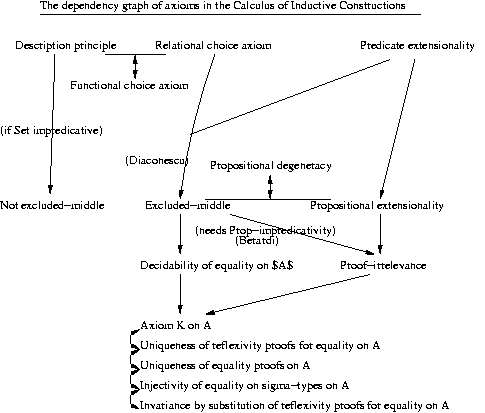
\includegraphics[width=1.0\textwidth]{axioms.png}
\else
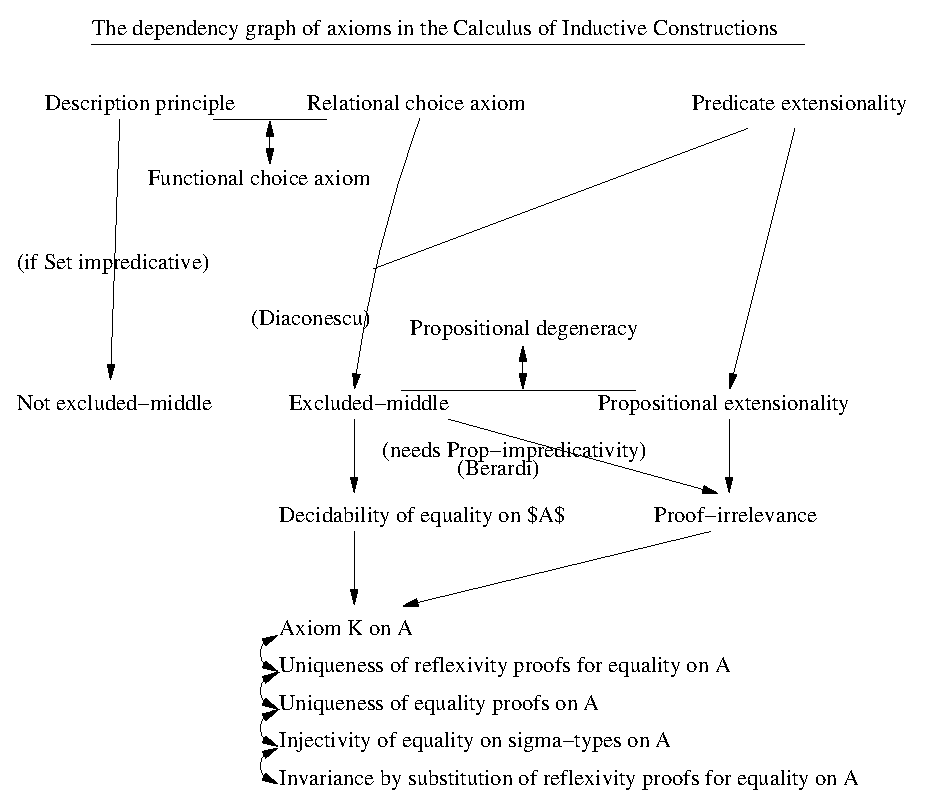
\includegraphics[width=1.0\textwidth]{axioms.eps}
\fi
%END LATEX

\Question{What standard axioms are inconsistent with {\Coq}?}

The axiom of unique choice together with classical logic
(e.g. excluded-middle) are inconsistent in the variant of the Calculus
of Inductive Constructions where {\Set} is impredicative.

As a consequence, the functional form of the axiom of choice and
excluded-middle, or any form of the axiom of choice together with
predicate extensionality are inconsistent in the {\Set}-impredicative
version of the Calculus of Inductive Constructions.

The main purpose of the \Set-predicative restriction of the Calculus
of Inductive Constructions is precisely to accommodate these axioms
which are quite standard in mathematical usage.

The $\Set$-predicative system is commonly considered consistent by
interpreting it in a standard set-theoretic boolean model, even with
classical logic, axiom of choice and predicate extensionality added.

\Question{What is Streicher's axiom $K$}
\label{Streicher}

Streicher's axiom $K$~\cite{HofStr98} is an axiom that asserts
dependent elimination of reflexive equality proofs.

\begin{coq_example*}
Axiom Streicher_K :
  forall (A:Type) (x:A) (P: x=x -> Prop),
    P (refl_equal x) -> forall p: x=x, P p.
\end{coq_example*}

In the general case, axiom $K$ is an independent statement of the
Calculus of Inductive Constructions.  However, it is true on decidable
domains (see file \vfile{\LogicEqdepDec}{Eqdep\_dec}). It is also
trivially a consequence of proof-irrelevance (see
\ref{proof-irrelevance}) hence of classical logic.

Axiom $K$ is equivalent to {\em Uniqueness of Identity Proofs} \cite{HofStr98}

\begin{coq_example*}
Axiom UIP : forall (A:Set) (x y:A) (p1 p2: x=y), p1 = p2.
\end{coq_example*}

Axiom $K$ is also equivalent to {\em Uniqueness of Reflexive Identity Proofs} \cite{HofStr98}

\begin{coq_example*}
Axiom UIP_refl : forall (A:Set) (x:A) (p: x=x), p = refl_equal x.
\end{coq_example*}

Axiom $K$ is also equivalent to 

\begin{coq_example*}
Axiom
  eq_rec_eq :
    forall (A:Set) (x:A) (P: A->Set) (p:P x) (h: x=x),
      p = eq_rect x P p x h.
\end{coq_example*}

It is also equivalent to the injectivity of dependent equality (dependent equality is itself equivalent to equality of dependent pairs).

\begin{coq_example*}
Inductive eq_dep (U:Set) (P:U -> Set) (p:U) (x:P p) :
forall q:U, P q -> Prop :=
    eq_dep_intro : eq_dep U P p x p x.
Axiom
  eq_dep_eq :
    forall (U:Set) (u:U) (P:U -> Set) (p1 p2:P u),
      eq_dep U P u p1 u p2 -> p1 = p2.
\end{coq_example*}

\Question{What is proof-irrelevance}
\label{proof-irrelevance}

A specificity of the Calculus of Inductive Constructions is to permit
statements about proofs. This leads to the question of comparing two
proofs of the same proposition. Identifying all proofs of the same
proposition is called {\em proof-irrelevance}:
$$
\forall A:\Prop, \forall p q:A, p=q
$$ 

Proof-irrelevance (in {\Prop}) can be assumed without contradiction in
{\Coq}. It expresses that only provability matters, whatever the exact
form of the proof is. This is in harmony with the common purely
logical interpretation of {\Prop}. Contrastingly, proof-irrelevance is
inconsistent in {\Set} since there are types in {\Set}, such as the
type of booleans, that are provably more than 2 elements.

Proof-irrelevance (in {\Prop}) is a consequence of classical logic
(see proofs in file \vfile{\LogicClassical}{Classical} and
\vfile{\LogicBerardi}{Berardi}). Proof-irrelevance is also a
consequence of propositional extensionality (i.e.  \coqtt{(A {\coqequiv} B)
{\coqimp} A=B}, see the proof in file
\vfile{\LogicClassicalFacts}{ClassicalFacts}).

Proof-irrelevance directly implies Streicher's axiom $K$.

\Question{What about functional extensionality?}

Extensionality of functions is admittedly consistent with the
Set-predicative Calculus of Inductive Constructions.

%\begin{coq_example*}
%  Axiom extensionality : (A,B:Set)(f,g:(A->B))(x:A)(f x)=(g x)->f=g.
%\end{coq_example*}

Let {\tt A}, {\tt B} be types. To deal with extensionality on 
\verb=A->B= without relying on a general extensionality axiom, 
a possible approach is to define one's own extensional equality on
\verb=A->B=.

\begin{coq_eval}
Variables A B : Set.
\end{coq_eval}

\begin{coq_example*}
Definition ext_eq (f g: A->B) := forall x:A, f x = g x.
\end{coq_example*}

and to reason on \verb=A->B= as a setoid (see the Chapter on
Setoids in the Reference Manual).

\Question{Is {\Prop} impredicative?}

Yes, the sort {\Prop} of propositions is {\em
impredicative}. Otherwise said, a statement of the form $\forall
A:Prop, P(A)$ can be instantiated by itself: if $\forall A:\Prop, P(A)$
is provable, then $P(\forall A:\Prop, P(A))$ is.

\Question{Is {\Set} impredicative?}

No, the sort {\Set} lying at the bottom of the hierarchy of
computational types is {\em predicative} in the basic {\Coq} system.
This means that a family of types in {\Set}, e.g. $\forall A:\Set, A
\rightarrow A$, is not a type in {\Set} and it cannot be applied on
itself.

However, the sort {\Set} was impredicative in the original versions of
{\Coq}. For backward compatibility, or for experiments by
knowledgeable users, the logic of {\Coq} can be set impredicative for
{\Set} by calling {\Coq} with the option {\tt -impredicative-set}.

{\Set} has been made predicative from version 8.0 of {\Coq}. The main
reason is to interact smoothly with a classical mathematical world
where both excluded-middle and the axiom of description are valid (see
file \vfile{\LogicClassicalDescription}{ClassicalDescription} for a
proof that excluded-middle and description implies the double negation
of excluded-middle in {\Set} and file {\tt Hurkens\_Set.v} from the
user contribution {\tt Rocq/PARADOXES} for a proof that
impredicativity of {\Set} implies the simple negation of
excluded-middle in {\Set}).

\Question{Is {\Type} impredicative?}

No, {\Type} is stratified. This is hidden for the
user, but {\Coq} internally maintains a set of constraints ensuring
stratification.

If {\Type} were impredicative then it would be possible to encode
Girard's systems $U-$ and $U$ in {\Coq} and it is known from Girard,
Coquand, Hurkens and Miquel that systems $U-$ and $U$ are inconsistent
[Girard 1972, Coquand 1991, Hurkens 1993, Miquel 2001]. This encoding
can be found in file {\tt Logic/Hurkens.v} of {\Coq} standard library.

For instance, when the user see {\tt $\forall$ X:Type, X->X : Type}, each
occurrence of {\Type} is implicitly bound to a different level, say
$\alpha$ and $\beta$ and the actual statement is {\tt
forall X:Type($\alpha$), X->X : Type($\beta$)} with the constraint
$\alpha<\beta$.

When a statement violates a constraint, the message {\tt Universe
inconsistency} appears. Example: {\tt fun (x:Type) (y:$\forall$ X:Type, X
{\coqimp} X) => y x x}.

\Question{I have two proofs of the same proposition. Can I prove they are equal?}

In the base {\Coq} system, the answer is generally no. However, if
classical logic is set, the answer is yes for propositions in {\Prop}.
The answer is also yes if proof irrelevance holds (see question
\ref{proof-irrelevance}).

There are also ``simple enough'' propositions for which you can prove
the equality without requiring any extra axioms.  This is typically
the case for propositions defined deterministically as a first-order
inductive predicate on decidable sets. See for instance in question
\ref{le-uniqueness} an axiom-free proof of the unicity of the proofs of
the proposition {\tt le m n} (less or equal on {\tt nat}).

%  It is an ongoing work of research to natively include proof
%  irrelevance in {\Coq}.

\Question{I have two proofs of an equality statement. Can I prove they are 
equal?}

 Yes, if equality is decidable on the domain considered (which
is the case for {\tt nat}, {\tt bool}, etc): see {\Coq} file
\verb=Eqdep_dec.v=). No otherwise, unless
assuming Streicher's axiom $K$ (see \cite{HofStr98}) or a more general
assumption such as proof-irrelevance (see \ref{proof-irrelevance}) or
classical logic.

All of these statements can be found in file \vfile{\LogicEqdep}{Eqdep}.

\Question{Can I prove that the second components of equal dependent
pairs are equal?}

 The answer is the same as for proofs of equality
statements. It is provable if equality on the domain of the first
component is decidable (look at \verb=inj_right_pair= from file
\vfile{\LogicEqdepDec}{Eqdep\_dec}), but not provable in the general
case. However, it is consistent (with the Calculus of Constructions)
to assume it is true. The file \vfile{\LogicEqdep}{Eqdep} actually
provides an axiom (equivalent to Streicher's axiom $K$) which entails
the result (look at \verb=inj_pair2= in \vfile{\LogicEqdep}{Eqdep}).

\subsection{Impredicativity}

\Question{Why {\tt injection} does not work on impredicative {\tt Set}?}

 E.g. in this case (this occurs only in the {\tt Set}-impredicative
 variant of \Coq):

\begin{coq_eval}
Reset Initial.
\end{coq_eval}

\begin{coq_example*}
Inductive I : Type :=
  intro : forall k:Set, k -> I.
Lemma eq_jdef : 
   forall x y:nat, intro _ x = intro _ y -> x = y.
Proof.
   intros x y H; injection H.
\end{coq_example*}

 Injectivity of constructors is restricted to predicative types. If
injectivity on large inductive types were not restricted, we would be
allowed to derive an inconsistency (e.g. following the lines of
Burali-Forti paradox). The question remains open whether injectivity
is consistent on some large inductive types not expressive enough to
encode known paradoxes (such as type I above).


\Question{What is a ``large inductive definition''?}

An inductive definition in {\Prop} or {\Set} is called large
if its constructors embed sets or propositions. As an example, here is
a large inductive type:

\begin{coq_example*}
Inductive sigST (P:Set -> Set) : Type :=
  existST : forall X:Set, P X -> sigST P.
\end{coq_example*}

In the {\tt Set} impredicative variant of {\Coq}, large inductive
definitions in {\tt Set} have restricted elimination schemes to
prevent inconsistencies. Especially, projecting the set or the
proposition content of a large inductive definition is forbidden. If
it were allowed, it would be possible to encode e.g. Burali-Forti
paradox \cite{Gir70,Coq85}.


%%%%%%%%%%%%%%%%%%%%%%%%%%%%%%%%%%%%%%%%%%%%%%%%%%%%%%%%%%%%%%%%%%%%%%
\section{Talkin' with the Rooster}


%%%%%%%
\subsection{My goal is ...,  how can I prove it?}


\Question{My goal is a conjunction, how can I prove it?}

Use some theorem or assumption or use the {\split} tactic.
\begin{coq_example}
Goal forall A B:Prop, A->B-> A/\B.
intros.
split.
assumption.
assumption.
Qed.
\end{coq_example}

\Question{My goal contains a conjunction as an hypothesis, how can I use it?}

If you want to decompose your hypothesis into other hypothesis you can use the {\decompose} tactic:

\begin{coq_example}
Goal forall A B:Prop, A/\B-> B.
intros.
decompose [and] H.
assumption.
Qed.
\end{coq_example}


\Question{My goal is a disjunction, how can I prove it?}

You can prove the left part or the right part of the disjunction using
{\left} or {\right} tactics. If you want to do a classical
reasoning step, use the {\tt classic} axiom to prove the right part with the assumption
that the left part of the disjunction is false.

\begin{coq_example}
Goal forall A B:Prop, A-> A\/B.
intros.
left.
assumption.
Qed.
\end{coq_example}

An example using classical reasoning:

\begin{coq_example}
Require Import Classical.

Ltac classical_right := 
match goal with 
| _:_ |-?X1 \/ _ => (elim (classic X1);intro;[left;trivial|right])
end.

Ltac classical_left := 
match goal with 
| _:_ |- _ \/?X1 => (elim (classic X1);intro;[right;trivial|left])
end.


Goal forall A B:Prop, (~A -> B) -> A\/B.
intros.
classical_right.
auto.
Qed.
\end{coq_example}

\Question{My goal is an universally quantified statement, how can I prove it?}

Use some theorem or assumption or introduce the quantified variable in
the context using the {\intro} tactic. If there are several
variables you can use the {\intros} tactic. A good habit is to
provide names for these variables: {\Coq} will do it anyway, but such
automatic naming decreases legibility and robustness.


\Question{My goal is an existential, how can I prove it?}

Use some theorem or assumption or exhibit the witness using the {\existstac} tactic.
\begin{coq_example}
Goal exists x:nat, forall y, x+y=y.
exists 0.
intros.
auto.
Qed.
\end{coq_example}


\Question{My goal is solvable by  some lemma, how can I prove it?}

Just use the {\apply} tactic.

\begin{coq_eval}
Reset Initial.
\end{coq_eval}

\begin{coq_example}
Lemma mylemma : forall x, x+0 = x.
auto.
Qed.

Goal 3+0 = 3.
apply mylemma.
Qed.
\end{coq_example}



\Question{My goal contains False as an hypothesis, how can I prove it?}

You can use the {\contradiction} or {\intuition} tactics.


\Question{My goal is an equality of two convertible terms, how can I prove it?}

Just use the {\reflexivity} tactic.

\begin{coq_example}
Goal forall x, 0+x = x.
intros.
reflexivity.
Qed.
\end{coq_example}

\Question{My goal is a {\tt let x := a in ...}, how can I prove it?}

Just use the {\intro} tactic.


\Question{My goal is a {\tt let (a, ..., b) := c in}, how can I prove it?}

Just use the {\destruct} c as (a,...,b) tactic.


\Question{My goal contains some existential hypotheses, how can I use it?}

You can use the tactic {\elim} with you hypotheses as an argument.

\Question{My goal contains some existential hypotheses, how can I use it and decompose my knowledge about this new thing into different hypotheses?}

\begin{verbatim}
Ltac DecompEx H P := elim H;intro P;intro TO;decompose [and] TO;clear TO;clear H.
\end{verbatim}


\Question{My goal is an equality, how can I swap the left and right hand terms?}

Just use the {\symmetry} tactic.
\begin{coq_example}
Goal forall x y : nat, x=y -> y=x.
intros.
symmetry.
assumption.
Qed.
\end{coq_example}

\Question{My hypothesis is an equality, how can I swap the left and right hand terms?}

Just use the {\symmetryin} tactic.

\begin{coq_example}
Goal forall x y : nat, x=y -> y=x.
intros.
symmetry in H.
assumption.
Qed.
\end{coq_example}


\Question{My goal is an equality, how can I prove it by transitivity?}

Just use the {\transitivity} tactic.
\begin{coq_example}
Goal forall x y z : nat, x=y -> y=z -> x=z.
intros.
transitivity y.
assumption.
assumption.
Qed.
\end{coq_example}


\Question{My goal would be solvable using {\tt apply;assumption} if it would not create meta-variables, how can I prove it?}

You can use {\tt eapply yourtheorem;eauto} but it won't work in all cases ! (for example if more than one hypothesis match one of the subgoals generated by \eapply) so you should rather use  {\tt try solve [eapply yourtheorem;eauto]}, otherwise some metavariables may be incorrectly instantiated.

\begin{coq_example}
Lemma trans : forall x y z : nat, x=y -> y=z -> x=z.
intros.
transitivity y;assumption.
Qed.

Goal forall x y z : nat, x=y -> y=z -> x=z.
intros.
eapply trans;eauto.
Qed.

Goal forall x y z t : nat, x=y -> x=t -> y=z -> x=z.
intros.
eapply trans;eauto.
Undo.
eapply trans.
apply H.
auto.
Qed.

Goal forall x y z t : nat, x=y -> x=t -> y=z -> x=z.
intros.
eapply trans;eauto.
Undo.
try solve [eapply trans;eauto].
eapply trans.
apply H.
auto.
Qed.

\end{coq_example}

\Question{My goal is solvable by  some lemma within a set of lemmas and I don't want to remember which one, how can I prove it?}

You can use a what is called a hints' base.

\begin{coq_example}
Require Import ZArith.
Require Ring.
Open Local Scope Z_scope.
Lemma toto1 : 1+1 = 2.
ring.
Qed.
Lemma toto2 : 2+2 = 4.
ring.
Qed.
Lemma toto3 : 2+1 = 3.
ring.
Qed.

Hint Resolve toto1 toto2 toto3 : mybase.

Goal 2+(1+1)=4. 
auto with mybase.
Qed.
\end{coq_example}


\Question{My goal is one of the hypotheses, how can I prove it?}

Use the {\assumption} tactic.

\begin{coq_example}
Goal 1=1 -> 1=1.
intro.
assumption.
Qed.
\end{coq_example}


\Question{My goal appears twice in the hypotheses and I want to choose which one is used, how can I do it?}

Use the {\exact} tactic.
\begin{coq_example}
Goal 1=1 -> 1=1 -> 1=1.
intros.
exact H0.
Qed.
\end{coq_example}

\Question{What can be the difference between applying one hypothesis or another in the context of the last question?}

From a proof point of view it is equivalent but if you want to extract
a program from your proof, the two hypotheses can lead to different
programs.


\Question{My goal is a propositional tautology, how can I prove it?}

Just use the {\tauto} tactic.
\begin{coq_example}
Goal forall A B:Prop, A-> (A\/B) /\ A.
intros.
tauto.
Qed.
\end{coq_example}

\Question{My goal is a first order formula, how can I prove it?}

Just use the semi-decision tactic: \firstorder.

\iffalse
todo: demander un exemple � Pierre
\fi

\Question{My goal is solvable by a sequence of rewrites, how can I prove it?}

Just use the {\congruence} tactic.
\begin{coq_example}
Goal forall a b c d e, a=d -> b=e -> c+b=d -> c+e=a.
intros.
congruence.
Qed.
\end{coq_example}


\Question{My goal is a disequality solvable by a sequence of rewrites, how can I prove it?}

Just use the {\congruence} tactic.

\begin{coq_example}
Goal forall a b c d, a<>d -> b=a -> d=c+b -> b<>c+b.
intros.
congruence.
Qed.
\end{coq_example}


\Question{My goal is an equality on some ring (e.g. natural numbers), how can I prove it?}

Just use the {\ring} tactic.

\begin{coq_example}
Require Import ZArith.
Require Ring.
Open Local Scope Z_scope.
Goal forall a b : Z, (a+b)*(a+b) = a*a + 2*a*b + b*b. 
intros.
ring.
Qed.
\end{coq_example}

\Question{My goal is an equality on some field (e.g. real numbers), how can I prove it?}

Just use the {\field} tactic.

\begin{coq_example}
Require Import Reals.
Require Ring.
Open Local Scope R_scope.
Goal forall a b : R, b*a<>0 -> (a/b) * (b/a) = 1. 
intros.
field.
assumption.
Qed.
\end{coq_example}


\Question{My goal is an inequality on integers in Presburger's arithmetic (an expression build from +,-,constants and variables), how can I prove it?}


\begin{coq_example}
Require Import ZArith.
Require Omega.
Open Local Scope Z_scope.
Goal forall a : Z, a>0 -> a+a > a. 
intros.
omega.
Qed.
\end{coq_example}


\Question{My goal is an equation solvable using equational hypothesis on some ring (e.g. natural numbers), how can I prove it?}

You need the {\gb} tactic (see Lo�c Pottier's homepage).

\subsection{Tactics usage}

\Question{I want to state a fact that I will use later as an hypothesis, how can I do it?}

If you want to use forward reasoning (first proving the fact and then
using it) you just need to use the {\assert} tactic. If you want to use
backward reasoning (proving your goal using an assumption and then
proving the assumption) use the {\cut} tactic.

\begin{coq_example}
Goal forall A B C D : Prop, (A -> B) -> (B->C) -> A -> C. 
intros.
assert (A->C).
intro;apply H0;apply H;assumption.
apply H2.
assumption.
Qed.

Goal forall A B C D : Prop, (A -> B) -> (B->C) -> A -> C. 
intros.
cut (A->C).
intro.
apply H2;assumption.
intro;apply H0;apply H;assumption.
Qed.
\end{coq_example}




\Question{I want to state a fact that I will use later as an hypothesis and prove it later, how can I do it?}

You can use {\cut} followed by {\intro} or you can use the following {\Ltac} command:
\begin{verbatim}
Ltac assert_later t := cut t;[intro|idtac]. 
\end{verbatim}

\Question{What is the difference between {\Qed} and {\Defined}?}

These two commands perform type checking, but when {\Defined} is used the new definition is set as transparent, otherwise it is defined as opaque (see \ref{opaque}).


\Question{How can I know what a tactic does?}

You can use the {\tt info} command.



\Question{Why {\auto} does not work? How can I fix it?}

You can increase the depth of the proof search or add some lemmas in the base of hints.
Perhaps you may need to use \eauto.

\Question{What is {\eauto}?}

This is the same tactic as \auto, but it relies on {\eapply} instead of \apply.

\iffalse
todo les espaces
\fi

\Question{How can I speed up {\auto}?}

You can use \texttt{info }\auto to replace {\auto} by the tactics it generates.
You can split your hint bases into smaller ones.


\Question{What is the equivalent of {\tauto} for classical logic?}

Currently there are no equivalent tactic for classical logic. You can use G�del's ``not not'' translation.


\Question{I want to replace some term with another in the goal, how can I do it?}

If one of your hypothesis (say {\tt H}) states that the terms are equal you can use the {\rewrite} tactic. Otherwise you can use the {\replace} {\tt with} tactic. 

\Question{I want to replace some term with another in an hypothesis, how can I do it?}

You can use the {\rewrite} {\tt in} tactic.

\Question{I want to replace some symbol with its definition, how can I do it?}

You can use the {\unfold} tactic.

\Question{How can I reduce some term?}

You can use the {\simpl} tactic.

\Question{How can I declare a shortcut for some term?}

You can use the {\set} or {\pose} tactics.

\Question{How can I perform case analysis?}

You can use the {\case} or {\destruct} tactics.

\Question{How can I prevent the case tactic from losing information ?}

You may want to use the (now standard) {\tt case\_eq} tactic. See the Coq'Art page 159.

\Question{Why should I name my intros?}

When you use the {\intro} tactic you don't have to give a name to your
hypothesis. If you do so the name will be generated by {\Coq} but your
scripts may be less robust. If you add some hypothesis to your theorem
(or change their order), you will have to change your proof to adapt
to the new names.

\Question{How can I automatize the naming?}

You can use the {\tt Show Intro.} or  {\tt Show Intros.} commands to generate the names and use your editor to generate a fully named {\intro} tactic. 
This can be automatized within {\tt xemacs}.

\begin{coq_example}
Goal forall A B C : Prop, A -> B -> C -> A/\B/\C.
Show Intros.
(*
A B C H H0
H1
*)
intros A B C H H0 H1.
repeat split;assumption.
Qed.
\end{coq_example}

\Question{I want to automatize the use of some tactic, how can I do it?}

You need to use the {\tt proof with T} command and add {\ldots} at the
end of your sentences.

For instance:
\begin{coq_example}
Goal forall A B C : Prop, A -> B/\C -> A/\B/\C.
Proof with assumption.
intros.
split...
Qed.
\end{coq_example}

\Question{I want to execute the {\texttt proof with} tactic only if it solves the goal, how can I do it?}

You need to use the {\try} and {\solve} tactics. For instance:
\begin{coq_example}
Require Import ZArith.
Require Ring.
Open Local Scope Z_scope.
Goal forall a b c : Z, a+b=b+a.
Proof with try solve [ring].
intros...
Qed.
\end{coq_example}

\Question{How can I do the opposite of the {\intro} tactic?}

You can use the {\generalize} tactic.

\begin{coq_example}
Goal forall A B : Prop, A->B-> A/\B.
intros.
generalize H.
intro.
auto.
Qed.
\end{coq_example}

\Question{One of the hypothesis is an equality between a variable and some term, I want to get rid of this variable, how can I do it?}

You can use the {\subst} tactic. This will rewrite the equality everywhere and clear the assumption.

\Question{What can I do if I get ``{\tt generated subgoal term has metavariables in it }''?}

You should use the {\eapply} tactic, this will generate some goals containing metavariables. 

\Question{How can I instantiate some metavariable?}

Just use the {\instantiate} tactic.


\Question{What is the use of the {\pattern} tactic?}

The {\pattern} tactic transforms the current goal, performing
beta-expansion on all the applications featuring this tactic's
argument. For instance, if the current goal includes a subterm {\tt
phi(t)}, then {\tt pattern t} transforms the subterm into {\tt (fun
x:A => phi(x)) t}. This can be useful when {\apply} fails on matching,
to abstract the appropriate terms.

\Question{What is the difference between assert, cut and generalize?}

PS: Notice for people that are interested in proof rendering that \assert
and {\pose} (and \cut) are not rendered the same as {\generalize} (see the
HELM experimental rendering tool at \ahref{http://helm.cs.unibo.it/library.html}{\url{http://helm.cs.unibo.it}}, link
HELM, link COQ Online). Indeed {\generalize} builds a beta-expanded term
while \assert, {\pose} and {\cut} uses a let-in.

\begin{verbatim}
  (* Goal is T *)
  generalize (H1 H2).
  (* Goal is A->T *)
  ... a proof of A->T ...
\end{verbatim}

is rendered into something like
\begin{verbatim}
  (h) ... the proof of A->T ...
      we proved A->T
  (h0) by (H1 H2) we proved A
  by (h h0) we proved T
\end{verbatim}
while 
\begin{verbatim}
  (* Goal is T *)
  assert q := (H1 H2).
  (* Goal is A *)
  ... a proof of A ...
  (* Goal is A |- T *)
  ... a proof of T ...
\end{verbatim}
is rendered into something like
\begin{verbatim}
  (q) ... the proof of A ...
      we proved A
  ... the proof of T ...
  we proved T
\end{verbatim}
Otherwise said, {\generalize} is not rendered in a forward-reasoning way,
while {\assert} is.

\Question{What can I do if \Coq can not infer some implicit argument ?}

You can state explicitely what this implicit argument is. See \ref{implicit}.

\Question{How can I explicit some implicit argument ?}\label{implicit}

Just use \texttt{A:=term} where \texttt{A} is the argument.

For instance if you want to use the existence of ``nil'' on nat*nat lists:
\begin{verbatim}
exists (nil (A:=(nat*nat))).
\end{verbatim}

\iffalse
\Question{Is there anyway to do pattern matching with dependent types?}

todo
\fi

\subsection{Proof management}


\Question{How can I change the order of the subgoals?}

You can use the {\Focus} command to concentrate on some goal. When the goal is proved you will see the remaining goals.

\Question{How can I change the order of the hypothesis?}

You can use the {\tt Move ... after} command.

\Question{How can I change the name of an hypothesis?}

You can use the {\tt Rename ... into} command.

\Question{How can I delete some hypothesis?}

You can use the {\tt Clear} command.

\Question{How can use a proof which is not finished?}

You can use the {\tt Admitted} command to state your current proof as an axiom.

\Question{How can I state a conjecture?}

You can use the {\tt Admitted} command to state your current proof as an axiom.

\Question{What is the difference between a lemma, a fact and a theorem?}

From {\Coq} point of view there are no difference. But some tools can
have a different behavior when you use a lemma rather than a
theorem. For instance {\tt coqdoc} will not generate documentation for
the lemmas within your development.

\Question{How can I organize my proofs?}

You can organize your proofs using the section mechanism of \Coq. Have
a look at the manual for further information.


%%%%%%%%%%%%%%%%%%%%%%%%%%%%%%%%%%%%%%%%%%%%%%%%%%%%%%%%%%%%%%%%%%%%%%%%%%%%%%%%%%%
\section{Inductive and Co-inductive types}

\subsection{General}

\Question{How can I prove that two constructors are different?}

You can use the {\discriminate} tactic.

\begin{coq_example}
Inductive toto : Set := | C1 : toto | C2 : toto.
Goal C1 <> C2.
discriminate.
Qed.
\end{coq_example}

\Question{During an inductive proof, how to get rid of impossible cases of an inductive definition?}

Use the {\inversion} tactic.


\Question{How can I prove that 2 terms in an inductive set are equal? Or different?}

Have a look at \coqtt{decide equality} and \coqtt{discriminate} in the \ahref{http://coq.inria.fr/doc/main.html}{Reference Manual}.

\Question{Why is the proof of \coqtt{0+n=n} on natural numbers
trivial but the proof of \coqtt{n+0=n} is not?}

 Since \coqtt{+} (\coqtt{plus}) on natural numbers is defined by analysis on its first argument

\begin{coq_example}
Print plus.
\end{coq_example}

{\noindent} The expression \coqtt{0+n} evaluates to \coqtt{n}. As {\Coq} reasons
modulo evaluation of expressions, \coqtt{0+n} and \coqtt{n} are
considered equal and the theorem \coqtt{0+n=n} is an instance of the
reflexivity of equality. On the other side, \coqtt{n+0} does not
evaluate to \coqtt{n} and a proof by induction on \coqtt{n} is
necessary to trigger the evaluation of \coqtt{+}.

\Question{Why is dependent elimination in Prop not
available by default?}

 
This is just because most of the time it is not needed. To derive a
dependent elimination principle in {\tt Prop}, use the command {\tt Scheme} and
apply the elimination scheme using the \verb=using= option of
\verb=elim=, \verb=destruct= or \verb=induction=.


\Question{Argh! I cannot write expressions like ``~{\tt if n <= p then p else n}~'', as in any programming language}
\label{minmax}

The short answer : You should use {\texttt le\_lt\_dec n p} instead.\\

That's right, you can't.
If you type for instance the following ``definition'':
\begin{coq_eval}
Reset Initial.
\end{coq_eval}
\begin{coq_example}
Definition max (n p : nat) := if n <= p then p else n.
\end{coq_example}

As \Coq~ says, the term ``~\texttt{n <= p}~'' is a proposition, i.e. a
statement that belongs to the mathematical world. There are many ways to
prove such a proposition, either by some computation, or using some already
proven theoremas. For instance, proving $3-2 \leq 2^{45503}$ is very easy,
using some theorems on arithmetical operations. If you compute both numbers
before comparing them, you risk to use a lot of time and space.


On the contrary, a function for computing the greatest of two natural numbers
is an algorithm  which, called on two natural numbers
$n$ and $p$, determines wether $n\leq p$ or $p < n$.
Such a function is a \emph{decision  procedure} for the inequality of
 \texttt{nat}.  The possibility of writing such a procedure comes 
directly from de decidability of the order $\leq$ on natural numbers.


When you write a piece of code like 
``~\texttt{if n <= p then \dots{} else \dots}~''
in a
programming language like \emph{ML} or \emph{Java}, a call to such a 
decision procedure is generated. The decision procedure is in general
a primitive function, written in a low-level language, in the correctness
of which you have to trust.

The standard Library of the system \emph{Coq} contains a  
(constructive) proof of decidability of the order $\leq$ on
\texttt{nat} : the function \texttt{le\_lt\_dec} of 
the module \texttt{Compare\_dec} of library \texttt{Arith}.

The following code shows how to define correctly \texttt{min} and
\texttt{max}, and prove some properties of these functions.

\begin{coq_example}
Require Import Compare_dec.

Definition max (n p : nat) := if le_lt_dec n p then p else n.

Definition min (n p : nat) := if le_lt_dec n p then n else p.

Eval compute in (min 4 7).

Theorem min_plus_max : forall n p, min n p + max n p  = n + p.
Proof.
 intros n p; 
 unfold min, max; 
 case (le_lt_dec n p);
 simpl; auto with arith.
Qed.

Theorem max_equiv : forall n p, max n p = p <-> n <= p.
Proof.
 unfold max; intros n p; case (le_lt_dec n p);simpl; auto.
 intuition auto with arith.
 split. 
 intro e; rewrite e; auto with arith.
 intro H; absurd (p < p); eauto with arith.
Qed.
\end{coq_example}

\Question{I wrote my own decision procedure for $\leq$, which
is much  faster than yours, but proving such theorems as
 \texttt{max\_equiv} seems to be quite difficult}

Your code is probably the following one:

\begin{coq_example}
Fixpoint my_le_lt_dec (n p :nat) {struct n}: bool  :=
 match n, p with 0, _ => true
               | S n', S p' => my_le_lt_dec n' p'
               | _   , _    => false
 end.

Definition my_max (n p:nat) := if my_le_lt_dec n p then p else n.

Definition my_min (n p:nat) := if my_le_lt_dec n p then n else p.
\end{coq_example}


For instance, the computation of \texttt{my\_max 567 321} is almost
immediate, whereas one can't wait for  the result of 
\texttt{max 56 32}, using \emph{Coq's} \texttt{le\_lt\_dec}.

This is normal. Your definition is a simple recursive function which
returns a boolean value. Coq's \texttt{le\_lt\_dec} is a \emph{certified
function}, i.e. a complex object, able not only to tell wether $n\leq p$
or $p<n$, but also of building a complete proof of the correct inequality.
What make \texttt{le\_lt\_dec} inefficient for computing \texttt{min}
and \texttt{max} is the building of a huge proof term.

Nevertheless,  \texttt{le\_lt\_dec} is very useful. Its type 
is a strong specification, using the
\texttt{sumbool} type (look at the reference manual or chapter 9 of
\cite{coqart}). Eliminations of the form
``~\texttt{case (le\_lt\_dec n p)}~'' provide proofs of
either $n \leq p$ or $p < n$, allowing to prove easily theorems as in
question~\ref{minmax}. Unfortunately, this not the case of your
\texttt{my\_le\_lt\_dec}, which returns a quite non-informative boolean
value.


\begin{coq_example}
Check le_lt_dec.
\end{coq_example}

You should keep in mind that \texttt{le\_lt\_dec} is useful to build
certified programs which need to compare natural numbers, and is not
designed to compare quickly two numbers.

Nevertheless, the \emph{extraction} of \texttt{le\_lt\_dec} towards 
\emph{Ocaml} or \emph{Haskell}, is a reasonable program for comparing two
natural numbers in Peano form in linear time.

It is also possible to keep your boolean function as a decision procedure,
but you have to establish yourself the relationship between \texttt{my\_le\_lt\_dec} and the propositions $n\leq p$ and $p<n$:

\begin{coq_example*}
Theorem my_le_lt_dec_true : 
    forall n p, my_le_lt_dec n p = true <-> n <= p.

Theorem  my_le_lt_dec_false : 
   forall n p, my_le_lt_dec n p = false <-> p < n.
\end{coq_example*}


\subsection{Recursion}

\Question{Why can't I define a non terminating program?}

 Because otherwise the decidability of the type-checking
algorithm (which involves evaluation of programs) is not ensured.  On
another side, if non terminating proofs were allowed, we could get a
proof of {\tt False}:

\begin{coq_example*}
(* This is fortunately not allowed! *)
Fixpoint InfiniteProof (n:nat) : False := InfiniteProof n.
Theorem Paradox : False.
Proof (InfiniteProof O).
\end{coq_example*}


\Question{Why only structurally well-founded loops are allowed?}

 The structural order on inductive types is a simple and
powerful notion of termination. The consistency of the Calculus of
Inductive Constructions relies on it and another consistency proof
would have to be made for stronger termination arguments (such
as the termination of the evaluation of CIC programs themselves!).

In spite of this, all non-pathological termination orders can be mapped
to a structural order. Tools to do this are provided in the file 
\vfile{\InitWf}{Wf} of the standard library of {\Coq}.

\Question{How to define loops based on non structurally smaller
recursive calls?}

 The procedure is as follows (we consider the definition of {\tt
mergesort} as an example).

\begin{itemize}

\item Define the termination order, say {\tt R} on the type {\tt A} of
the arguments of the loop.

\begin{coq_eval}
Open Scope R_scope.
Require Import List.
\end{coq_eval}

\begin{coq_example*}
Definition R (a b:list nat) := length a < length b.
\end{coq_example*}

\item Prove that this order is well-founded (in fact that all elements in {\tt A} are accessible along {\tt R}).

\begin{coq_example*}
Lemma Rwf : well_founded R.
\end{coq_example*}

\item Define the step function (which needs proofs that recursive
calls are on smaller arguments).

\begin{coq_example*}
Definition split (l : list nat) 
   : {l1: list nat | R l1 l} * {l2 : list nat | R l2 l}
   := (* ... *) .
Definition concat (l1 l2 : list nat) : list nat := (* ... *) .
Definition merge_step (l : list nat) (f: forall l':list nat, R l' l -> list nat) :=
  let (lH1,lH2) := (split l) in
  let (l1,H1) := lH1 in
  let (l2,H2) := lH2 in
  concat (f l1 H1) (f l2 H2).
\end{coq_example*}

\item Define the recursive function by fixpoint on the step function.

\begin{coq_example*}
Definition merge := Fix Rwf (fun _ => list nat) merge_step.
\end{coq_example*}

\end{itemize}

\Question{What is behind the accessibility and well-foundedness proofs?}

 Well-foundedness of some relation {\tt R} on some type {\tt A}
is defined as the accessibility of all elements of {\tt A} along {\tt R}.

\begin{coq_example}
Print well_founded.
Print Acc.
\end{coq_example}

The structure of the accessibility predicate is a well-founded tree
branching at each node {\tt x} in {\tt A} along all the nodes {\tt x'}
less than {\tt x} along {\tt R}. Any sequence of elements of {\tt A}
decreasing along the order {\tt R} are branches in the accessibility
tree. Hence any decreasing along {\tt R} is mapped into a structural
decreasing in the accessibility tree of {\tt R}. This is emphasised in
the definition of {\tt fix} which recurs not on its argument {\tt x:A}
but on the accessibility of this argument along {\tt R}.

See file \vfile{\InitWf}{Wf}.

\Question{How to perform simultaneous double induction?}

 In general a (simultaneous) double induction is simply solved by an
induction on the first hypothesis followed by an inversion over the
second hypothesis. Here is an example

\begin{coq_eval}
Reset Initial.
\end{coq_eval}

\begin{coq_example}
Inductive even : nat -> Prop :=
  | even_O : even 0
  | even_S : forall n:nat, even n -> even (S (S n)).

Inductive odd : nat -> Prop :=
  | odd_SO : odd 1
  | odd_S : forall n:nat, odd n -> odd (S (S n)).

Lemma not_even_and_odd : forall n:nat, even n -> odd n -> False.
induction 1.
  inversion 1.
  inversion 1. apply IHeven; trivial.
\end{coq_example}
\begin{coq_eval}
Qed.
\end{coq_eval}

In case the type of the second induction hypothesis is not
dependent, {\tt inversion} can just be replaced by {\tt destruct}.

\Question{How to define a function by simultaneous double recursion?}

 The same trick applies, you can even use the pattern-matching
compilation algorithm to do the work for you. Here is an example:

\begin{coq_example}
Fixpoint minus (n m:nat) {struct n} : nat :=
  match n, m with
  | O, _ => 0
  | S k, O => S k
  | S k, S l => minus k l
  end.
Print  minus.
\end{coq_example}

In case of dependencies in the type of the induction objects
$t_1$ and $t_2$, an extra argument stating $t_1=t_2$ must be given to
the fixpoint definition

\Question{How to perform nested and double induction?}

 To reason by nested (i.e. lexicographic) induction, just reason by
induction on the successive components.

\smallskip

Double induction (or induction on pairs) is a restriction of the
lexicographic induction. Here is an example of double induction.

\begin{coq_example}
Lemma nat_double_ind : 
forall P : nat -> nat -> Prop, P 0 0 -> 
  (forall m n, P m n -> P m (S n)) -> 
  (forall m n, P m n -> P (S m) n) -> 
     forall m n, P m n.
intros P H00 HmS HSn; induction m.
(* case 0 *)
induction n; [assumption | apply HmS; apply IHn].
(* case Sm *)
intro n; apply HSn; apply IHm.
\end{coq_example}
\begin{coq_eval}
Qed.
\end{coq_eval}

\Question{How to define a function by nested recursion?}

 The same trick applies. Here is the example of Ackermann
function.

\begin{coq_example}
Fixpoint ack (n:nat) : nat -> nat :=
  match n with
  | O => S
  | S n' =>
     (fix ack' (m:nat) : nat :=
        match m with
        | O => ack n' 1
        | S m' => ack n' (ack' m')
        end)
  end.
\end{coq_example}


\subsection{Co-inductive types}

\Question{I have a cofixpoint $t:=F(t)$ and I want to prove $t=F(t)$. How to do it?}

Just case-expand $F({\tt t})$ then complete by a trivial case analysis.
Here is what it gives on e.g. the type of streams on naturals

\begin{coq_eval}
Set Implicit Arguments.
\end{coq_eval}
\begin{coq_example}
CoInductive Stream (A:Set) : Set :=
  Cons : A -> Stream A -> Stream A.
CoFixpoint nats (n:nat) : Stream nat := Cons n (nats (S n)).
Lemma Stream_unfold : 
   forall n:nat, nats n = Cons n (nats (S n)).
Proof.
  intro;
  change (nats n = match nats n with
                  | Cons x s => Cons x s
                  end).
  case (nats n); reflexivity.
Qed.
\end{coq_example}



\section{Syntax and notations}

\Question{I do not want to type ``forall'' because it is too long, what can I do?}

You can define your own notation for forall:
\begin{verbatim}
Notation "fa x : t, P" := (forall x:t, P) (at level 200, x ident).
\end{verbatim}
or if your are using {\CoqIde} you can define a pretty symbol for for all and an input method (see \ref{forallcoqide}).



\Question{How can I define a notation for square?}

You can use for instance:
\begin{verbatim}
Notation "x ^2" := (Rmult x x) (at level 20).
\end{verbatim}
Note that you can not use:
\begin{texttt}
Notation "x $^�$" := (Rmult x x) (at level 20).
\end{texttt}
because ``$^2$'' is an iso-latin character. If you really want this kind of notation you should use UTF-8.


\Question{Why ``no associativity'' and  ``left associativity'' at the same level does not work?}

Because we relie on camlp4 for syntactical analysis and camlp4 does not really implement no associativity. By default, non associative operators are defined as right associative.



\Question{How can I know the associativity associated with a level?}

You can do ``Print Grammar constr'', and decode the output from camlp4, good luck !

\section{Modules}




%%%%%%%
\section{\Ltac}

\Question{What is {\Ltac}?}

{\Ltac} is the tactic language for \Coq. It provides the user with a
high-level ``toolbox'' for tactic creation.

\Question{Why do I always get the same error message?}


\Question{Is there any printing command in {\Ltac}?}

You can use the {\idtac} tactic with a string argument. This string
will be printed out. The same applies to the {\fail} tactic

\Question{What is the syntax for let in {\Ltac}?}

If $x_i$ are identifiers and $e_i$ and $expr$ are tactic expressions, then let reads:
\begin{center}
{\tt let $x_1$:=$e_1$ with $x_2$:=$e_2$\ldots with $x_n$:=$e_n$ in
$expr$}.
\end{center}
Beware that if $expr$ is complex (i.e. features at least a sequence) parenthesis
should be added around it. For example: 
\begin{coq_example}
Ltac twoIntro := let x:=intro in (x;x).
\end{coq_example}

\Question{What is the syntax for pattern matching in {\Ltac}?}

Pattern matching on a term $expr$ (non-linear first order unification)
with patterns $p_i$ and tactic expressions $e_i$ reads:
\begin{center}
\hspace{10ex}
{\tt match $expr$ with
\hspace*{2ex}$p_1$ => $e_1$
\hspace*{1ex}\textbar$p_2$ => $e_2$
\hspace*{1ex}\ldots
\hspace*{1ex}\textbar$p_n$ => $e_n$
\hspace*{1ex}\textbar\ \textunderscore\ => $e_{n+1}$
end.
}
\end{center}
Underscore matches all terms.

\Question{What is the semantics for ``match goal''?}

The semantics of {\tt match goal} depends on whether it returns
tactics or not.  The {\tt match goal} expression matches the current
goal against a series of patterns: {$hyp_1 {\ldots} hyp_n$ \textbar-
$ccl$}. It uses a first-order unification algorithm and in case of
success, if the right-hand-side is an expression, it tries to type it
while if the right-hand-side is a tactic, it tries to apply it.  If the
typing or the tactic application fails, the {\tt match goal} tries all
the possible combinations of $hyp_i$ before dropping the branch and
moving to the next one. Underscore matches all terms.

\Question{Why can't I use a ``match goal'' returning a tactic in a non
tail-recursive position?}

This is precisely because the semantics of {\tt match goal} is to
apply the tactic on the right as soon as a pattern unifies what is
meaningful only in tail-recursive uses.

The semantics in non tail-recursive call could have been the one used
for terms (i.e. fail if the tactic expression is not typable, but
don't try to apply it). For uniformity of semantics though, this has
been rejected.

\Question{How can I generate a new name?}

You can use the following syntax:
{\tt let id:=fresh in \ldots}\\
For example:
\begin{coq_example}
Ltac introIdGen := let id:=fresh in intro id.
\end{coq_example}


\iffalse
\Question{How can I access the type of a term?}

You can use typeof.
todo
\fi

\Question{How can I define static and dynamic code?}

\section{Tactics written in Ocaml}

\Question{Can you show me an example of a tactic written in OCaml?}

You have some examples of tactics written in Ocaml in the ``contrib'' directory of {\Coq} sources. 




\section{Case studies}


\Question{How can I define vectors or lists of size n?}

\Question{How to prove that 2 sets are different?}

 You need to find a property true on one set and false on the
other one. As an example we show how to prove that {\tt bool} and {\tt
nat} are discriminable. As discrimination property we take the
property to have no more than 2 elements.

\begin{coq_example*}
Theorem nat_bool_discr : bool <> nat.
Proof.
  pose (discr :=
    fun X:Set =>
      ~ (forall a b:X, ~ (forall x:X, x <> a -> x <> b -> False))).
  intro Heq; assert (H: discr bool).
  intro H; apply (H true false); destruct x; auto.
  rewrite Heq in H; apply H; clear H.
  destruct a; destruct b as [|n]; intro H0; eauto.
  destruct n; [ apply (H0 2); discriminate | eauto ].
Qed.
\end{coq_example*}

\Question{Is there an axiom-free proof of Streicher's axiom $K$ for
the equality on {\tt nat}?}
\label{K-nat}

Yes, because equality is decidable on {\tt nat}. Here is the proof.

\begin{coq_example*}
Require Import Eqdep_dec.
Require Import Peano_dec.
Theorem K_nat :
  forall (x:nat) (P:x = x -> Prop), P (refl_equal x) -> forall p:x = x, P p.
Proof.
intros; apply K_dec_set with (p := p).
apply eq_nat_dec.
assumption.
Qed.
\end{coq_example*}

Similarly, we have

\begin{coq_example*}
Theorem eq_rect_eq_nat :
  forall (p:nat) (Q:nat->Type) (x:Q p) (h:p=p), x = eq_rect p Q x p h.
Proof.
intros; apply K_nat with (p := h); reflexivity.
Qed.
\end{coq_example*}

\Question{How to prove that two proofs of {\tt n<=m} on {\tt nat} are equal?}
\label{le-uniqueness}

This is provable without requiring any axiom because axiom $K$
directly holds on {\tt nat}. Here is a proof using question \ref{K-nat}.

\begin{coq_example*}
Require Import Arith.
Scheme le_ind' := Induction for le Sort Prop.
Theorem le_uniqueness_proof : forall (n m : nat) (p q : n <= m), p = q.
Proof.
induction p using le_ind'; intro q.
 replace (le_n n) with
  (eq_rect _ (fun n0 => n <= n0) (le_n n) _ (refl_equal n)).
 2:reflexivity.
  generalize (refl_equal n).
    pattern n at 2 4 6 10, q; case q; [intro | intros m l e].
     rewrite <- eq_rect_eq_nat; trivial.
     contradiction (le_Sn_n m); rewrite <- e; assumption.
 replace (le_S n m p) with
  (eq_rect _ (fun n0 => n <= n0) (le_S n m p) _ (refl_equal (S m))).
 2:reflexivity.
  generalize (refl_equal (S m)).
    pattern (S m) at 1 3 4 6, q; case q; [intro Heq | intros m0 l HeqS].
     contradiction (le_Sn_n m); rewrite Heq; assumption.
     injection HeqS; intro Heq; generalize l HeqS.
      rewrite <- Heq; intros; rewrite <- eq_rect_eq_nat.
      rewrite (IHp l0); reflexivity.
Qed.
\end{coq_example*}

\Question{How to exploit equalities on sets}

To extract information from an equality on sets, you need to
find a predicate of sets satisfied by the elements of the sets. As an
example, let's consider the following theorem.

\begin{coq_example*}
Theorem interval_discr :
  forall m n:nat,
    {x : nat | x <= m} = {x : nat | x <= n} -> m = n.
\end{coq_example*}

We have a proof requiring the axiom of proof-irrelevance. We
conjecture that proof-irrelevance can be circumvented by introducing a
primitive definition of discrimination of the proofs of
\verb!{x : nat | x <= m}!.

\begin{latexonly}%
The proof can be found in file {\tt interval$\_$discr.v} in this directory.
%Here is the proof
%\begin{small}
%\begin{flushleft}
%\begin{texttt}
%\def_{\ifmmode\sb\else\subscr\fi}
%\include{interval_discr.v}
%%% WARNING semantics of \_ has changed !
%\end{texttt}
%$a\_b\_c$
%\end{flushleft}
%\end{small}
\end{latexonly}%
\begin{htmlonly}%
\ahref{./interval_discr.v}{Here} is the proof.
\end{htmlonly}

\Question{I have a problem of dependent elimination on
proofs, how to solve it?}

\begin{coq_eval}
Reset Initial.
\end{coq_eval}

\begin{coq_example*}
Inductive Def1 : Set := c1 : Def1.
Inductive DefProp : Def1 -> Prop :=
  c2 : forall d:Def1, DefProp d.
Inductive Comb : Set :=
  c3 : forall d:Def1, DefProp d -> Comb.
Lemma eq_comb :
  forall (d1 d1':Def1) (d2:DefProp d1) (d2':DefProp d1'),
    d1 = d1' -> c3 d1 d2 = c3 d1' d2'.
\end{coq_example*}

 You need to derive the dependent elimination
scheme for DefProp by hand using {\coqtt Scheme}.

\begin{coq_eval}
Abort.
\end{coq_eval}

\begin{coq_example*}
Scheme DefProp_elim := Induction for DefProp Sort Prop.
Lemma eq_comb :
  forall d1 d1':Def1,
    d1 = d1' ->
    forall (d2:DefProp d1) (d2':DefProp d1'), c3 d1 d2 = c3 d1' d2'.
intros.
destruct H.
destruct d2 using DefProp_elim.
destruct d2' using DefProp_elim.
reflexivity.
Qed.
\end{coq_example*}


\Question{And what if I want to prove the following?}

\begin{coq_example*}
Inductive natProp : nat -> Prop :=
  | p0 : natProp 0
  | pS : forall n:nat, natProp n -> natProp (S n).
Inductive package : Set :=
  pack : forall n:nat, natProp n -> package.
Lemma eq_pack :
 forall n n':nat,
   n = n' ->
   forall (np:natProp n) (np':natProp n'), pack n np = pack n' np'.
\end{coq_example*}



\begin{coq_eval}
Abort.
\end{coq_eval}
\begin{coq_example*}
Scheme natProp_elim := Induction for natProp Sort Prop.
Definition pack_S : package -> package.
destruct 1.
apply (pack (S n)).
apply pS; assumption.
Defined.
Lemma eq_pack :
  forall n n':nat,
    n = n' ->
    forall (np:natProp n) (np':natProp n'), pack n np = pack n' np'.
intros n n' Heq np np'.
generalize dependent n'.
induction np using natProp_elim.
induction np' using natProp_elim; intros; auto.
 discriminate Heq.
induction np' using natProp_elim; intros; auto.
 discriminate Heq.
change (pack_S (pack n np) = pack_S (pack n0 np')).
apply (f_equal (A:=package)).
apply IHnp.
auto.
Qed.
\end{coq_example*}







\section{Publishing tools}

\Question{How can I generate some latex from my development?}

You can use {\tt coqdoc}.

\Question{How can I generate some HTML from my development?}

You can use {\tt coqdoc}.

\Question{How can I generate some dependency graph from my development?}

\Question{How can I cite some {\Coq} in my latex document?}

You can use {\tt coq\_tex}.

\Question{How can I cite the {\Coq} reference manual?}

You can use this bibtex entry:
\begin{verbatim}
@Manual{Coq:manual,
  title =        {The Coq proof assistant reference manual},
  author =       {\mbox{The Coq development team}},
  organization = {LogiCal Project},
  note =         {Version 8.0},
  year =         {2004},
  url =          "http://coq.inria.fr"
}
\end{verbatim}

\Question{Where can I publish my developments in {\Coq}?}

You can submit your developments as a user contribution to the {\Coq}
development team. This ensures its liveness along the evolution and
possible changes of {\Coq}.

You can also submit your developments to the HELM/MoWGLI repository at
the University of Bologna (see
\ahref{http://mowgli.cs.unibo.it}{\url{http://mowgli.cs.unibo.it}}). For
developments submitted in this database, it is possible to visualize
the developments in natural language and execute various retrieving
requests.

\Question{How can I read my proof in natural language?}

You can submit your proof to the HELM/MoWGLI repository and use the
rendering tool provided by the server (see
\ahref{http://mowgli.cs.unibo.it}{\url{http://mowgli.cs.unibo.it}}).

\section{\CoqIde}

\Question{What is {\CoqIde}?}

{\CoqIde} is a gtk based GUI for \Coq.

\Question{How to enable Emacs keybindings?}
 Insert \texttt{gtk-key-theme-name = "Emacs"}
    in your \texttt{.coqide-gtk2rc} file. It may be in the current dir
    or in \verb#$HOME# dir. This is done by default.

%$ juste pour que la coloration emacs marche

\Question{How to enable antialiased fonts?}

 Set the \verb#GDK_USE_XFT# variable to \verb#1#. This is by default with \verb#Gtk >= 2.2#.
    If some of your fonts are not available, set \verb#GDK_USE_XFT# to \verb#0#.

\Question{How to use those Forall and Exists pretty symbols?}\label{forallcoqide}
 Thanks to the notation features in \Coq, you just need to insert these
lines in your {\Coq} buffer:\\
\begin{texttt}
Notation "$\forall$ x : t, P" := (forall x:t, P) (at level 200, x ident).
\end{texttt}\\
\begin{texttt}
Notation "$\exists$ x : t, P" := (exists x:t, P) (at level 200, x ident).
\end{texttt}

Copy/Paste of these lines from this file will not work outside of \CoqIde.
You need to load a file containing these lines or to enter the $\forall$
using an input method (see \ref{inputmeth}). To try it just use \verb#Require Import utf8# from inside
\CoqIde. 
To enable these notations automatically start coqide with
\begin{verbatim}
	coqide -l utf8
\end{verbatim}
In the ide subdir of {\Coq} library, you will find a sample utf8.v with some 
pretty simple notations.

\Question{How to define an input method for non ASCII symbols?}\label{inputmeth}

\begin{itemize}
\item First solution: type \verb#<CONTROL><SHIFT>2200# to enter a forall in the script widow. 
	2200 is the hexadecimal code for forall in unicode charts and is encoded as 	
	in UTF-8.
	2203 is for exists. See \ahref{http://www.unicode.org}{\url{http://www.unicode.org}} for more codes.
\item Second solution: rebind \verb#<AltGr>a# to forall and \verb#<AltGr>e# to exists. 
	Under X11, you need to use something like
\begin{verbatim}
		xmodmap -e "keycode  24 = a A F13 F13" 
		xmodmap -e "keycode  26 = e E F14 F14"
\end{verbatim}
	and then to add   
\begin{verbatim}
		bind "F13" {"insert-at-cursor" ("")}
		bind "F14" {"insert-at-cursor" ("")}
\end{verbatim}
	to your "binding "text"" section in \verb#.coqiderc-gtk2rc.#
	The strange ("") argument is the UTF-8 encoding for
	0x2200. 
	You can compute these encodings using the lablgtk2 toplevel with 
\begin{verbatim}		
Glib.Utf8.from_unichar 0x2200;;
\end{verbatim}
	Further symbols can be bound on higher Fxx keys or on even on other keys you
	do not need .
\end{itemize}

\Question{How to build a custom {\CoqIde} with user ml code?}
 Use 
	coqmktop -ide -byte m1.cmo...mi.cmo
    or 
	coqmktop -ide -opt m1.cmx...mi.cmx

\Question{How to customize the shortcuts for menus?}
 Two solutions are offered:
\begin{itemize}
\item Edit \$HOME/.coqide.keys by hand or
\item Add "gtk-can-change-accels = 1" in your .coqide-gtk2rc file. Then
    from \CoqIde, you may select a menu entry and press the desired 
    shortcut. 
\end{itemize}

\Question{What encoding should I use? What is this $\backslash$x\{iiii\} in my file?}
 The encoding option is related to the way files are saved. 
 Keep it as UTF-8 until it becomes important for you to exchange files 
 with non UTF-8 aware applications.
 If you choose something else than UTF-8, then missing characters will 
 be encoded by $\backslash$x\{....\} or $\backslash$x\{........\}
 where each dot is an hex. digit. 
 The number between braces is the hexadecimal UNICODE index for the
  missing character.
    



\section{Extraction}

\Question{What is program extraction?}

Program extraction consist in generating a program from a constructive proof.

\Question{Which language can I extract to?}

You can extract your programs to Objective Caml and Haskell.

\Question{How can I extract an incomplete proof?}

You can provide programs for your axioms.



%%%%%%%
\section{Glossary}

\Question{Can you explain me what an evaluable constant is?}

An evaluable constant is a constant which is unfoldable.

\Question{What is a goal?}

The goal is the statement to be proved.

\Question{What is a meta variable?}

A meta variable in {\Coq} represents a ``hole'', i.e. a part of a proof
that is still unknown. 

\Question{What is Gallina?}  

Gallina is the specification language of \Coq. Complete documentation
of this language can be found in the Reference Manual.

\Question{What is The Vernacular?}  

It is the language of commands of Gallina i.e. definitions, lemmas, {\ldots}  


\Question{What is a dependent type?}

A dependant type is a type which depends on some term. For instance
``vector of size n'' is a dependant type representing all the vectors
of size $n$. Its type depends on $n$

\Question{What is a proof by reflection?}

This is a proof generated by some computation which is done using the
internal reduction of {\Coq} (not using the tactic language of {\Coq}
(\Ltac) nor the implementation language for \Coq).  An example of
tactic using the reflection mechanism is the {\ring} tactic. The
reflection method consist in reflecting a subset of {\Coq} language (for
example the arithmetical expressions) into an object of the \Coq
language itself (in this case an inductive type denoting arithmetical
expressions).  For more information see~\cite{howe,harrison,boutin}
and the last chapter of the Coq'Art.

\Question{What is intuitionistic logic?}

This is any logic which does not assume that ``A or not A''.


\Question{What is proof-irrelevance?}

See question \ref{proof-irrelevance}


\Question{What is the difference between opaque and transparent?}{\label{opaque}}	

Opaque definitions can not be unfolded but transparent ones can.


\section{Troubleshooting}

\Question{What can I do when {\tt Qed.} is slow?}

Sometime you can use the {\abstracttac} tactic, which makes as if you had
stated some local lemma, this speeds up the typing process.

\Question{Why \texttt{Reset Initial.} does not work when using \texttt{coqc}?}

The initial state corresponds to the state of coqtop when the interactive
session began. It does not make sense in files to compile.


\Question{What can I do if I get ``No more subgoals but non-instantiated existential variables''?}

This means that {\eauto} or {\eapply} didn't instantiate an
existential variable which eventually got erased by some computation.
You have to backtrack to the faulty occurrence of {\eauto} or
{\eapply} and give the missing argument an explicit value.

Note that you can see what the current existential are using the {\tt
  Show Existentials} command.

\begin{coq_example}
Lemma example_show_existentials :  forall a b c:nat, a=b -> b=c -> a=c.
Proof.
intros.
eapply trans_equal.
Show Existentials.
eassumption.
assumption.
Qed.
\end{coq_example}


\Question{What can I do if I get ``Cannot solve a second-order unification problem''?}

You can help {\Coq} using the {\pattern} tactic.

\Question{Why does {\Coq} tell me that \texttt{\{x:A|(P x)\}} is not convertible with \texttt{(sig A P)}?}

 This is because \texttt{\{x:A|P x\}} is a notation for
\texttt{sig (fun x:A => P x)}. Since {\Coq} does not reason up to
$\eta$-conversion, this is different from \texttt{sig P}.


\Question{I copy-paste a term and {\Coq} says it is not convertible
  to the original term. Sometimes it even says the copied term is not
well-typed.}

 This is probably due to invisible implicit information (implicit
arguments, coercions and Cases annotations) in the printed term, which
is not re-synthesised from the copied-pasted term in the same way as
it is in the original term.

  Consider for instance {\tt (@eq Type True True)}. This term is
printed as {\tt True=True} and re-parsed as {\tt (@eq Prop True
True)}. The two terms are not convertible (hence they fool tactics
like {\tt pattern}).

  There is currently no satisfactory answer to the problem. However,
the command {\tt Set Printing All} is useful for diagnosing the
problem.
 
  Due to coercions, one may even face type-checking errors. In some
rare cases, the criterion to hide coercions is a bit too loose, which
may result in a typing error message if the parser is not able to find
again the missing coercion.



\section{Conclusion and Farewell.}
\label{ccl}

\Question{What if my question isn't answered here?} 
\label{lastquestion}

Don't panic \verb+:-)+. You can try the {\Coq} manual~\cite{Coq:manual} for a technical
description of the prover. The Coq'Art~\cite{Coq:coqart} is the first
book written on {\Coq} and provides a comprehensive review of the
theorem prover as well as a number of example and exercises. Finally,
the tutorial~\cite{Coq:Tutorial} provides a smooth introduction to
theorem proving in \Coq.


%%%%%%%
\newpage
\nocite{LaTeX:intro}
\nocite{LaTeX:symb}
\bibliography{fk}

%%%%%%%
\typeout{*********************************************}
\typeout{********* That makes \thequestion{\space} questions **********}
\typeout{*********************************************}

\end{document}
